\documentclass[12pt,t]{beamer}
% \documentclass[t]{beamer}
\usepackage[utf8]{inputenc}
\usepackage[catalan]{babel}
\usepackage{verbatim}
\usepackage{hyperref}
\usepackage{amsfonts,amssymb,amsmath,amsthm, wasysym, multirow}
\usepackage{listings}
\lstset{language=R}
\usepackage[T1]{fontenc}        
\usepackage{pgf}
\usepackage{epsdice}
\usepackage{pgfpages}


\usepackage{tikz}
\usetikzlibrary{arrows,shapes,plotmarks,backgrounds,trees}
\newcounter{nivell}
\setcounter{nivell}{0}
\newcommand{\nounivell}{%
  \addtocounter{nivell}{1}}
\newcommand{\nvl}{\value{nivell}}
\tikzstyle{hyb}=[rectangle,fill=green!50,draw]%,minimum size=0.5mm]
\tikzstyle{tree}=[circle,fill=green!50,draw]%,minimum size=0.5mm]

\tikzstyle{hybgr}=[rectangle,fill=green!50,draw,minimum size=5mm]
\tikzstyle{treegr}=[circle,fill=green!50,draw,minimum size=5.5mm]

\tikzstyle{hybnou}=[rectangle,fill=red!50,draw]%,minimum size=0.5mm]
\tikzstyle{trenou}=[circle,fill=red!50,draw]%,minimum size=0.5mm]

\tikzstyle{treered}=[circle,fill=red!50,draw]%,minimum size=6mm]


\newcommand{\etq}[1]{%
\draw (#1) node {\scriptsize $#1$};
}
\newcommand{\etqb}[2]{%
\draw (#1) node {\scriptsize $#1_{#2}$};
}
%\usetikzlibrary{arrows,shapes,plotmarks,backgrounds,trees,positioning}
%\usetikzlibrary{decorations.pathmorphing,calc,snakes}
%\usepackage{marvosym}
%
\usetheme[hideothersubsections,left]{Marburg}
\usecolortheme{sidebartab}
\useinnertheme[shadow]{rounded}
% \useoutertheme[footline=empty,subsection=true,compress]{infolines}
% \useoutertheme[footline=empty,subsection=true,compress]{miniframes}
% \usefonttheme{serif}

\setbeamertemplate{caption}[numbered]
\setbeamertemplate{navigation symbols}{}


\newcommand{\red}[1]{\textcolor{red}{#1}}
\newcommand{\green}[1]{\textcolor{green}{#1}}
\newcommand{\blue}[1]{\textcolor{blue}{#1}}
\newcommand{\gray}[1]{\textcolor{gray}{#1}}
\renewcommand{\emph}[1]{{\color{red}#1}}

\setbeamertemplate{frametitle}
{\begin{centering}
\medskip
\color{blue}
\textbf{\insertframetitle}
\medskip
\end{centering}
}
\usecolortheme{rose}
\usecolortheme{dolphin}
\mode<presentation>


\newcommand{\CC}{\mathbb{C}}
\newcommand{\RR}{\mathbb{R}}
\newcommand{\ZZ}{\mathbb{Z}}
\newcommand{\NN}{\mathbb{N}}
\newcommand{\KK}{\mathbb{K}}
\newcommand{\MM}{\mathcal{M}}
%\newcommand{\dbinom}{\displaystyle\binom}

\newcommand{\limn}{{\displaystyle \lim_{n\to\infty}}}
\renewcommand{\leq}{\leqslant}
\renewcommand{\geq}{\geqslant}
\def\tendeix{{\displaystyle\mathop{\longrightarrow}_{\scriptscriptstyle
n\to\infty}}}

\newcommand{\matriu}[1]{\left(\begin{matrix} #1 \end{matrix}\right)}

% \newcommand{\qed}{\hbox{}\nobreak\hfill\vrule width 1.4mm height 1.4mm depth 0mm
%     \par \goodbreak  skip}
%
% %
\theoremstyle{plain}
\newtheorem{teorema}{Teorema}
\newtheorem{prop}{Proposició}
\newtheorem{cor}{Coro\l.lari}
\theoremstyle{definition}
\newtheorem{exemple}{Exemple}
\newtheorem{defin}{Definició}
\newtheorem{obs}{Observació}

\newcounter{seccions}
\newcommand{\seccio}[1]{\addtocounter{seccions}{1}
\medskip\par\noindent\emph{\theseccions.
#1} skip\par }

\newcommand{\EM}{\Omega}
\newcommand{\PP}{\mathcal{P}}

\title[\red{Matemàtiques III}]{}
\author[]{}
\date{}



\begin{document}
\beamertemplatedotitem

\lstset{backgroundcolor=\color{green!50}}
\lstset{breaklines=true}
\lstset{basicstyle=\ttfamily}
\lstset{extendedchars=true}
\lstset{showstringspaces=false}

\begin{frame}
\vfill
\begin{center}
\gray{\LARGE Agrupaments (\textsl{Clustering})}
\end{center}
\vfill
\end{frame}

\section{Clustering}
\subsection{Introducció}
\begin{frame}
\frametitle{Introducció}

\blue{\bf Problema:} Donat un conjunt d'objectes, classificar-los en grups (\emph{clusters})  basant-nos en les seves semblances i diferències
\medskip

Algunes aplicacions en biologia:
\begin{itemize}
\item Classificació jeràrquica d'organismes (relacionada amb una filogènia)

\item Agrupament de gens amb pautes d'expressió similars

\item Agrupament de gens per semblança seqüencial

\item Agrupament de proteïnes per semblança estructural
\end{itemize}
\end{frame}

\begin{frame}
\frametitle{Principis bàsics}

\blue{\bf Homogeneïtat:} Objectes dins el mateix cluster han de ser propers (semblants)
\medskip

\blue{\bf Separació:} Objectes dins clusters diferents han de ser llunyans
\vspace*{-4ex}

\begin{center}
\begin{tabular}{ccc}
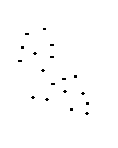
\includegraphics[width=0.3 \linewidth]{cluster1.pdf}
&
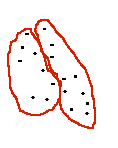
\includegraphics[width=0.3 \linewidth]{cluster1dolent.pdf}
&
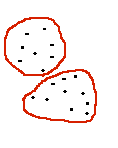
\includegraphics[width=0.3 \linewidth]{cluster1bo.pdf}
\\ & dolent & bo
\end{tabular}
\end{center}
Com formalitzar i calcular aquests principis intuïtius?

\end{frame}

\begin{frame}
\frametitle{Tipus de clustering}

\begin{itemize}
\item \emph{De partició:} Dividim els objectes en un nombre prefixat de clusters; possiblement provam diversos nombres de clusters i ens quedam amb el millor 
\end{itemize}
\vspace*{-2ex}

\begin{center}
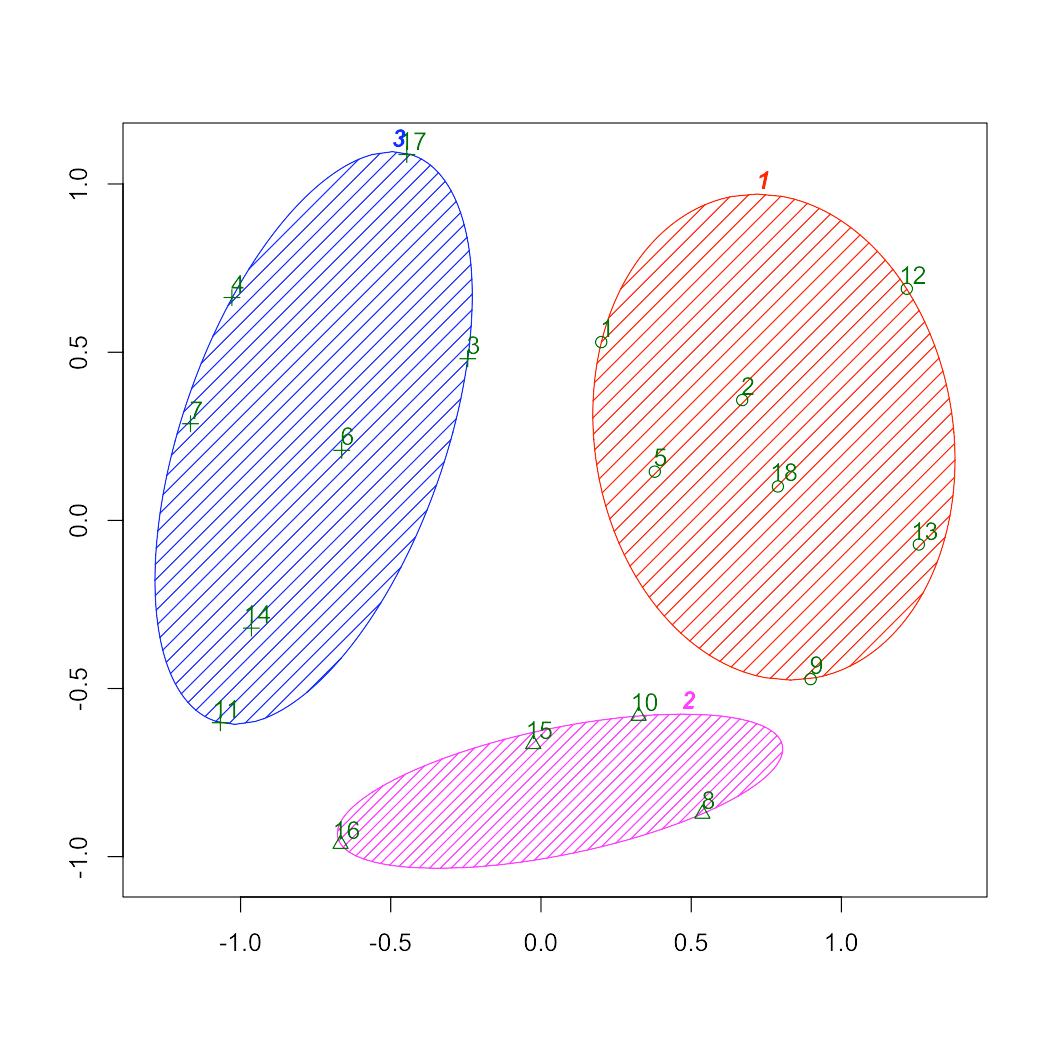
\includegraphics[width=0.65\linewidth]{Rplot7.pdf}
\end{center}




\end{frame}



\begin{frame}
\frametitle{Tipus de clustering}

\begin{itemize}
\item \emph{Jeràrquic}: Successivament agrupam (\emph{aglomeratius}) o dividim (\emph{divisius}) objectes o grups d'objectes. Produeix un arbre de classificació on els objectes pertanyen a clusters inclosos dins clusters inclosos dins clusters \ldots
\end{itemize}
\begin{center}
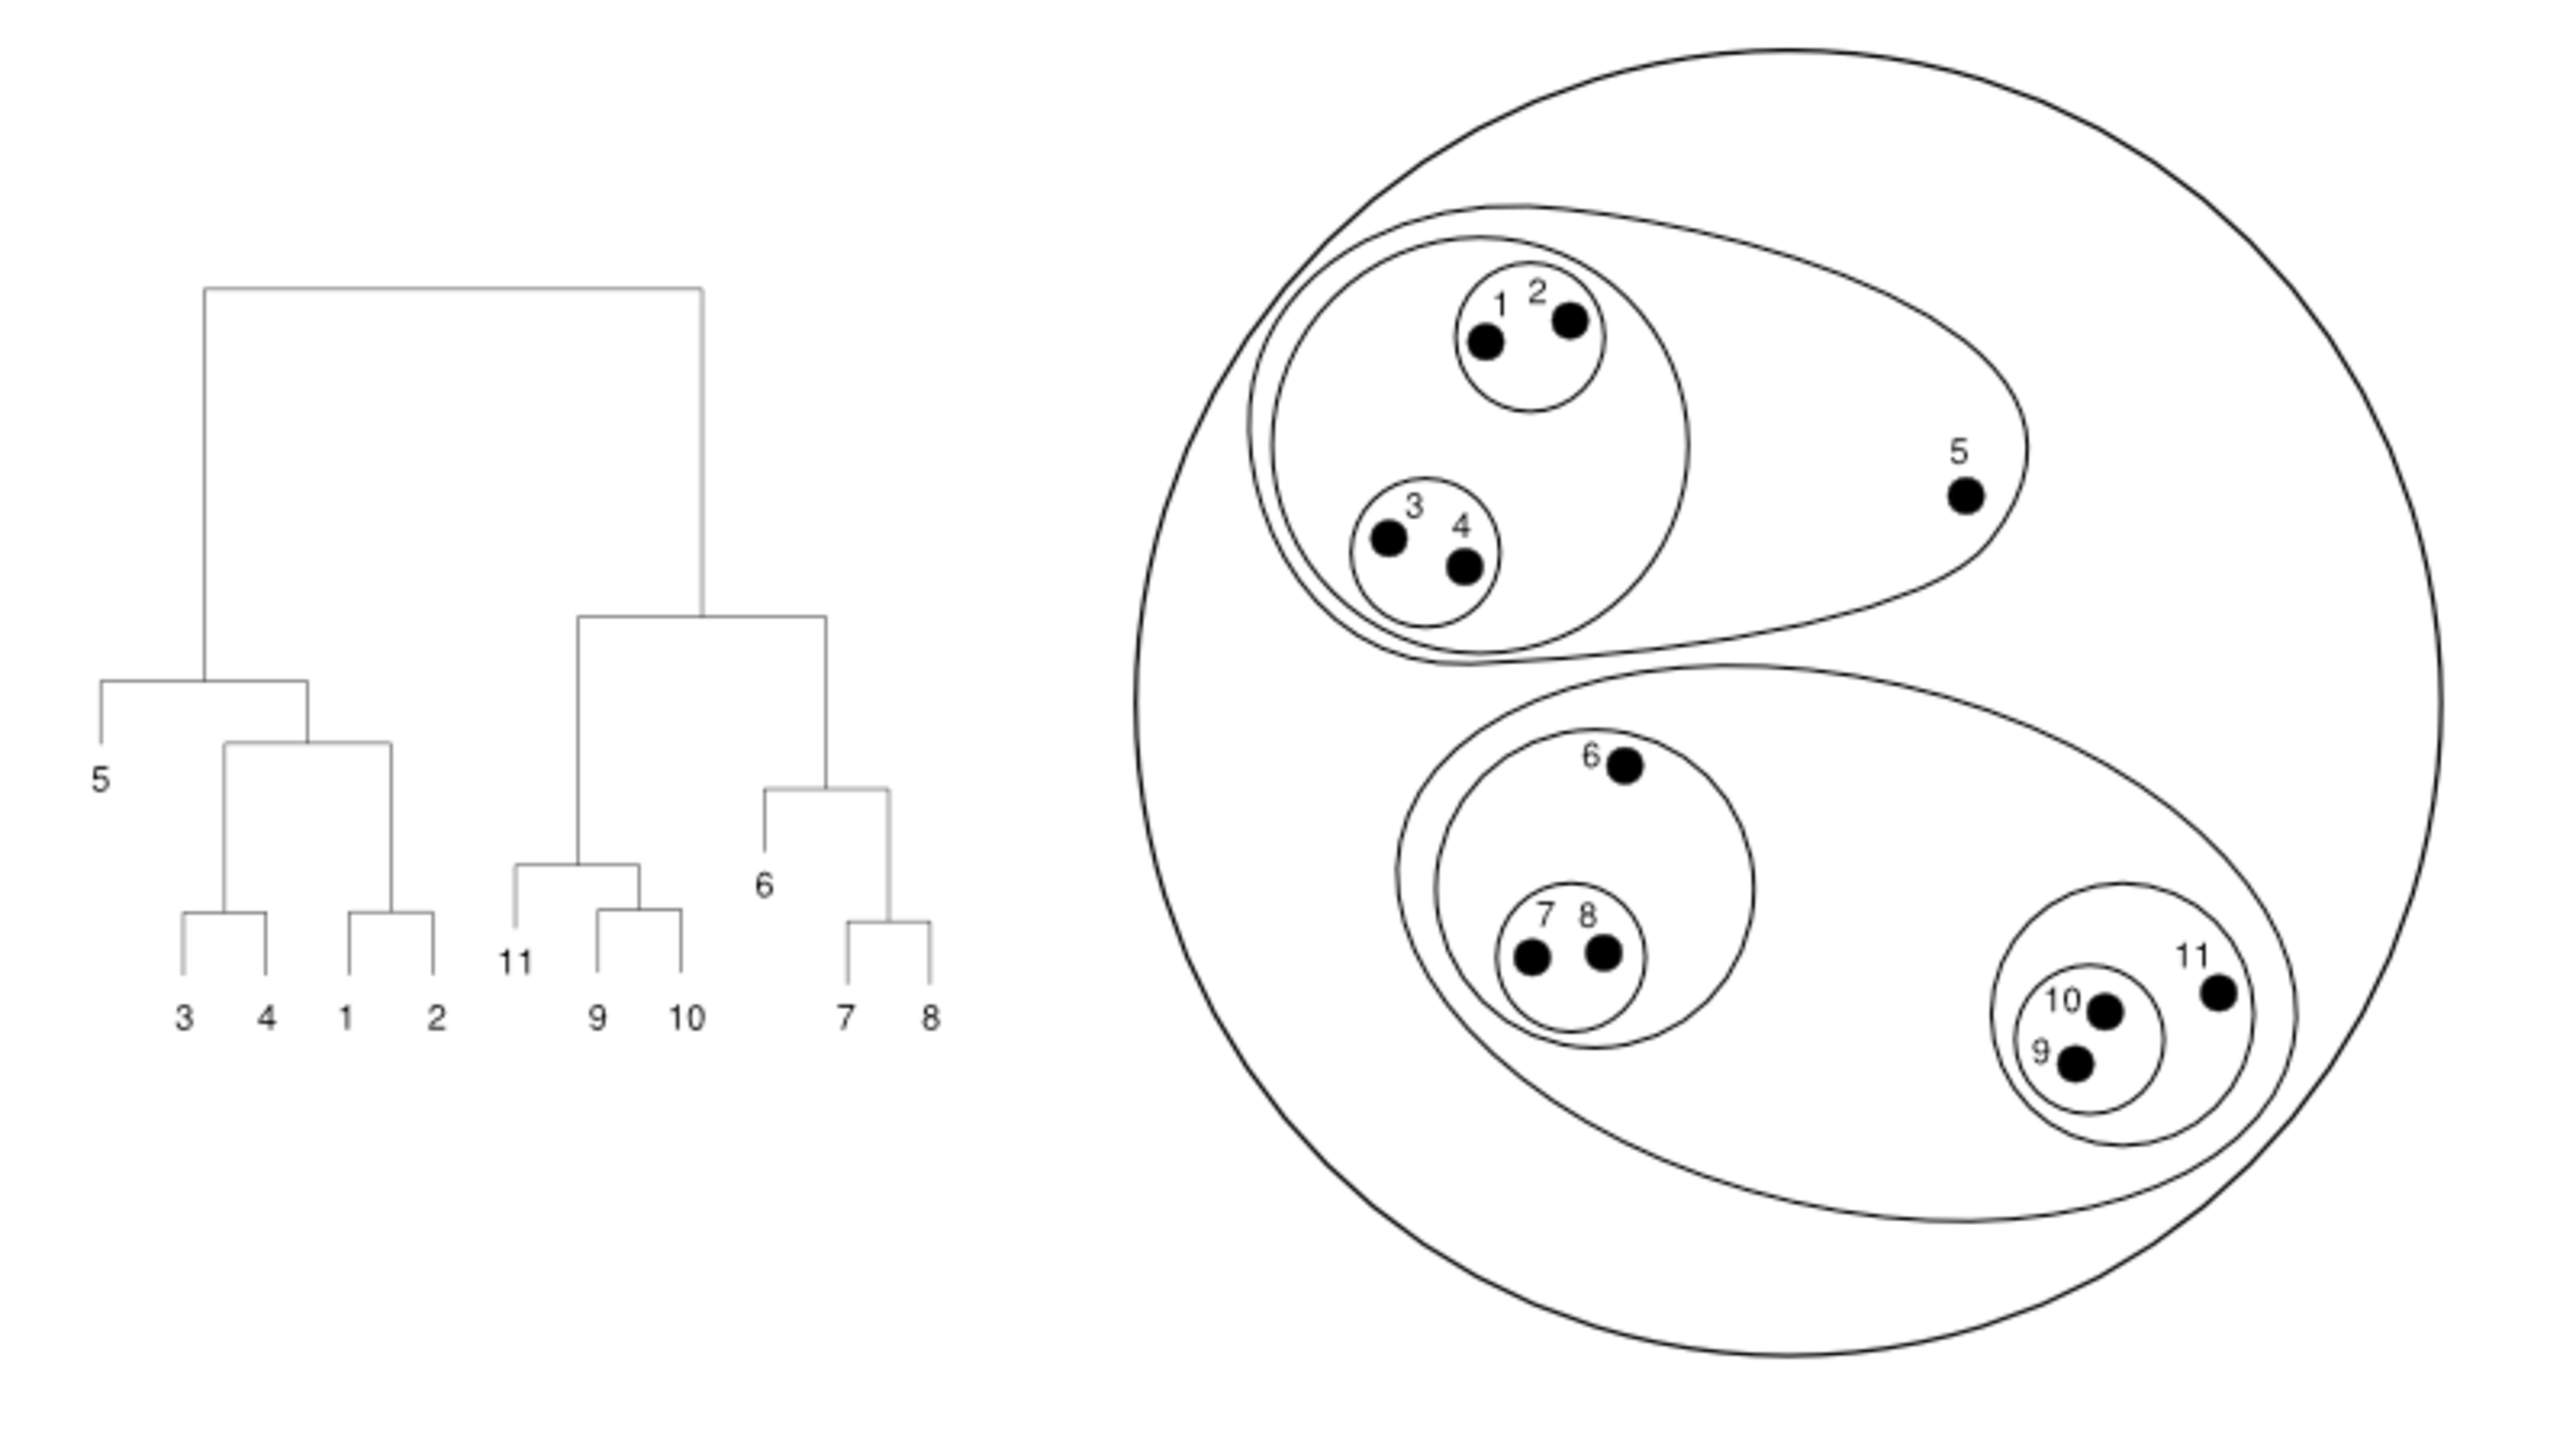
\includegraphics[width=0.7\linewidth]{hclust-example}
\end{center}




\end{frame}




\subsection{$k$-means}

\begin{frame}
\frametitle{$k$-means}

L'algoritme de les $k$-mitjanes (\emph{$k$-means}) cerca una partició del conjunt d'objectes, representats com a elements d'un espai $\RR^n$, en un nombre fixat $k$ de clusters
\medskip

Aquests clusters s'identifiquen per mitjà dels seus punts mitjans (\textsl{means})\pause
\vspace*{0.8cm}

Recordau que donat $\mathbf{x}=(x_1,\ldots,x_n)\in \RR^n$,
$$
\|\mathbf{x}\|=\sqrt{\sum_{i=1}^n x_i^2}
$$
i que donats $\mathbf{x},\mathbf{y} \in \RR^n$, $\|\mathbf{x}-\mathbf{y}\|$ és la \emph{distància euclidiana} entre 
$\mathbf{x}$ i $\mathbf{y}$.
\end{frame}


\begin{frame}
\frametitle{$k$-means}
Fixem el nombre de clusters $k$
\medskip

Donats punts $\mathbf{x}_1,\ldots,\mathbf{x}_p\in \RR^n$, l'objectiu és trobar $k$ punts $\mathbf{c}_1,\ldots,\mathbf{c}_k\in \RR^n$ que minimitzin
$$
\red{SS_C}(\mathbf{x}_1,\ldots,\mathbf{x}_p; k)=\sum_{i=1}^p\min_{j=1,\ldots,k} \|\mathbf{x}_i-\mathbf{c}_j\|^2
$$
Aleshores cada $\mathbf{c}_j$ definirà el cluster format pels $\mathbf{x}_i$ que estan més a prop d'ell que de cap altre $\mathbf{c}_l$:
$$
C_j=\{\mathbf{x}_i\mid \|\mathbf{x}_i-\mathbf{c}_j\|<\|\mathbf{x}_i-\mathbf{c}_l\|\mbox{ per a tot }l\neq j\}
$$
i
$$
SS_C(\mathbf{x}_1,\ldots,\mathbf{x}_p; k)=\sum_{j=1}^k\sum_{\mathbf{x}_i\in C_j}  \|\mathbf{x}_i-\mathbf{c}_j\|^2
$$

\end{frame}


\begin{frame}
\frametitle{$k$-means: Algoritme de Lloyd}
\vspace*{-3ex}

\begin{enumerate}
\item Escollim $\mathbf{c}_1,\ldots,\mathbf{c}_k$ (com vulguem)
\medskip

\item Assignam cada punt $\mathbf{x}_i$ al cluster $C_j$ definit pel centre $\mathbf{c}_j$ més proper
\medskip

\item Substituïm cada centre $\mathbf{c}_j$ pel punt mitjà del seu cluster $C_j$:
\vspace*{-1ex}

$$
\mathbf{c}_j= \Big(\sum_{\mathbf{x}_i\in C_j} \mathbf{x}_i\Big)/|C_j|
$$
\vspace*{-2ex}

\item Es repeteixen (2)--(3) fins que els clusters estabilitzen, o un nombre prefixat d'iteracions
\end{enumerate}
El resultat depèn dels $\mathbf{c}_1,\ldots,\mathbf{c}_k$ inicials.
\medskip

Aquest algoritme no té perquè donar un clustering òptim. Convé repetir-lo diverses vegades amb diferents inicialitzacions.


\end{frame}


\begin{frame}
\frametitle{Exemple}
\begin{center}
\begin{tikzpicture}[thick,>=stealth,scale=2]
\filldraw [black] (0.8, 1.3) circle (1pt);  
\filldraw [black] (0.8 , 1.8) circle (1pt);  
\filldraw [black] (1.0,0.9) circle (1pt);  
\filldraw [black] (1.1,0.1) circle (1pt);  
\filldraw [black] (1.1, 1.6) circle (1pt);  
\filldraw [black] (1.4, 0.6) circle (1pt);  
\filldraw [black] (1.5 ,0.1) circle (1pt);  
\filldraw [black] (2 ,2.1) circle (1pt);  
\filldraw [black] (1.5,2.3) circle (1pt);  
\filldraw [black] (1.8,1.8) circle (1pt);  
\filldraw [black] (2.3,0.5) circle (1pt);  
\filldraw [black] (0.3,2.2) circle (1pt);  
\filldraw [black] (1,2.5) circle (1pt);  
\filldraw [black] (2,0.5) circle (1pt);  
\filldraw [black] (2,1.5) circle (1pt);  
\filldraw [black] (2.5,1) circle (1pt);  
\filldraw [black] (0.5,0.5) circle (1pt);  
\filldraw [black] (1,2) circle (1pt);  
\draw (0,-0.2)--(0,3);
\draw (-0.2,0)--(3,0);
\draw (0.5,0)--(0.5,-0.1);
\draw (0.5,-0.2) node {\footnotesize 0.5};
\draw (1,0)--(1,-0.1);
\draw (1,-0.2) node {\footnotesize 1};
\draw (1.5,0)--(1.5,-0.1);
\draw (1.5,-0.2) node {\footnotesize 1.5};
\draw (2,0)--(2,-0.1);
\draw (2,-0.2) node {\footnotesize 2};
\draw (2.5,0)--(2.5,-0.1);
\draw (2.5,-0.2) node {\footnotesize 2.5};
\draw (-0.1,0.5)--(0,0.5);
\draw (-0.2,0.5) node {\footnotesize 0.5};
\draw (-0.1,1)--(0,1);
\draw (-0.2,1) node {\footnotesize 1};
\draw (-0.1,1.5)--(0,1.5);
\draw (-0.2,1.5) node {\footnotesize 1.5};
\draw (-0.1,2)--(0,2);
\draw (-0.2,2) node {\footnotesize 2};
\draw (-0.1,2.5)--(0,2.5);
\draw (-0.2,2.5) node {\footnotesize 2.5};
\pause
%\filldraw [black] (1.5,0) rectangle (1,1);  
%\filldraw [black] (1.5,1.5) rectangle (1,1);  
%\filldraw [black] (1.5,3) rectangle (1,1);  
%\draw (1.5,0) node[rectangle,fill=green!50,draw] {};
\draw (1.5,0) node[rectangle,fill=red,draw] {};
\draw (1.5,1.5) node[rectangle,fill=blue,draw] {};
\draw (1.5,3) node[rectangle,fill=green,draw] {};
\end{tikzpicture}
\end{center}
\end{frame}

\begin{frame}
\frametitle{Exemple}
\begin{center}
\begin{tikzpicture}[thick,>=stealth,scale=2]
\filldraw [red] (1.1,0.1) circle (1pt);  
\filldraw [red] (1.4, 0.6) circle (1pt);  
\filldraw [red] (1.5 ,0.1) circle (1pt);  
\filldraw [red] (2.3,0.5) circle (1pt);  
\filldraw [red] (2,0.5) circle (1pt);  
\filldraw [red] (0.5,0.5) circle (1pt);  
\filldraw [blue] (0.8, 1.3) circle (1pt);  
\filldraw [blue] (0.8 , 1.8) circle (1pt);  
\filldraw [blue] (1.0,0.9) circle (1pt);  
\filldraw [blue] (1.1, 1.6) circle (1pt);  
\filldraw [blue] (2 ,2.1) circle (1pt);  
\filldraw [blue] (1.8,1.8) circle (1pt);  
\filldraw [blue] (0.3,2.2) circle (1pt);  
\filldraw [blue] (2,1.5) circle (1pt);  
\filldraw [blue] (2.5,1) circle (1pt);  
\filldraw [blue] (1,2) circle (1pt);  
\filldraw [green] (1,2.5) circle (1pt);  
\filldraw [green] (1.5,2.3) circle (1pt);  
\draw (0,-0.2)--(0,3);
\draw (-0.2,0)--(3,0);
\draw (0.5,0)--(0.5,-0.1);
\draw (0.5,-0.2) node {\footnotesize 0.5};
\draw (1,0)--(1,-0.1);
\draw (1,-0.2) node {\footnotesize 1};
\draw (1.5,0)--(1.5,-0.1);
\draw (1.5,-0.2) node {\footnotesize 1.5};
\draw (2,0)--(2,-0.1);
\draw (2,-0.2) node {\footnotesize 2};
\draw (2.5,0)--(2.5,-0.1);
\draw (2.5,-0.2) node {\footnotesize 2.5};
\draw (-0.1,0.5)--(0,0.5);
\draw (-0.2,0.5) node {\footnotesize 0.5};
\draw (-0.1,1)--(0,1);
\draw (-0.2,1) node {\footnotesize 1};
\draw (-0.1,1.5)--(0,1.5);
\draw (-0.2,1.5) node {\footnotesize 1.5};
\draw (-0.1,2)--(0,2);
\draw (-0.2,2) node {\footnotesize 2};
\draw (-0.1,2.5)--(0,2.5);
\draw (-0.2,2.5) node {\footnotesize 2.5};
\draw (1.5,0) node[rectangle,fill=red,draw] {};
\draw (1.5,1.5) node[rectangle,fill=blue,draw] {};
\draw (1.5,3) node[rectangle,fill=green,draw] {};
%\draw (2.266667, 0.6666667) node[rectangle,fill=red,draw] {};
%\draw (1.100000, 0.4400000) node[rectangle,fill=blue,draw] {};
%\draw (1.230000, 1.9100000) node[rectangle,fill=green,draw] {};
\end{tikzpicture}
\end{center}
\end{frame}

\begin{frame}
\frametitle{Exemple}
\begin{center}
\begin{tikzpicture}[thick,>=stealth,scale=2]
\filldraw [red] (1.1,0.1) circle (1pt);  
\filldraw [red] (1.4, 0.6) circle (1pt);  
\filldraw [red] (1.5 ,0.1) circle (1pt);  
\filldraw [red] (2.3,0.5) circle (1pt);  
\filldraw [red] (2,0.5) circle (1pt);  
\filldraw [red] (0.5,0.5) circle (1pt);  
\filldraw [blue] (0.8, 1.3) circle (1pt);  
\filldraw [blue] (0.8 , 1.8) circle (1pt);  
\filldraw [blue] (1.0,0.9) circle (1pt);  
\filldraw [blue] (1.1, 1.6) circle (1pt);  
\filldraw [blue] (2 ,2.1) circle (1pt);  
\filldraw [blue] (1.8,1.8) circle (1pt);  
\filldraw [blue] (0.3,2.2) circle (1pt);  
\filldraw [blue] (2,1.5) circle (1pt);  
\filldraw [blue] (2.5,1) circle (1pt);  
\filldraw [blue] (1,2) circle (1pt);  
\filldraw [green] (1,2.5) circle (1pt);  
\filldraw [green] (1.5,2.3) circle (1pt);  
\draw (0,-0.2)--(0,3);
\draw (-0.2,0)--(3,0);
\draw (0.5,0)--(0.5,-0.1);
\draw (0.5,-0.2) node {\footnotesize 0.5};
\draw (1,0)--(1,-0.1);
\draw (1,-0.2) node {\footnotesize 1};
\draw (1.5,0)--(1.5,-0.1);
\draw (1.5,-0.2) node {\footnotesize 1.5};
\draw (2,0)--(2,-0.1);
\draw (2,-0.2) node {\footnotesize 2};
\draw (2.5,0)--(2.5,-0.1);
\draw (2.5,-0.2) node {\footnotesize 2.5};
\draw (-0.1,0.5)--(0,0.5);
\draw (-0.2,0.5) node {\footnotesize 0.5};
\draw (-0.1,1)--(0,1);
\draw (-0.2,1) node {\footnotesize 1};
\draw (-0.1,1.5)--(0,1.5);
\draw (-0.2,1.5) node {\footnotesize 1.5};
\draw (-0.1,2)--(0,2);
\draw (-0.2,2) node {\footnotesize 2};
\draw (-0.1,2.5)--(0,2.5);
\draw (-0.2,2.5) node {\footnotesize 2.5};
\draw (1.4667,0.3833) node[rectangle,fill=red,draw] {};
\draw (1.34,1.62) node[rectangle,fill=blue,draw] {};
\draw (1.26,2.41) node[rectangle,fill=green,draw] {};
%\draw (2.266667, 0.6666667) node[rectangle,fill=red,draw] {};
%\draw (1.100000, 0.4400000) node[rectangle,fill=blue,draw] {};
%\draw (1.230000, 1.9100000) node[rectangle,fill=green,draw] {};
\end{tikzpicture}
\end{center}
\end{frame}


\begin{frame}
\frametitle{Exemple}
\begin{center}
\begin{tikzpicture}[thick,>=stealth,scale=2]
\filldraw [blue] (0.8, 1.3) circle (1pt);  
\filldraw [blue] (0.8 , 1.8) circle (1pt);  
\filldraw [red] (1.0,0.9) circle (1pt);  
\filldraw [red] (1.1,0.1) circle (1pt);  
\filldraw [blue] (1.1, 1.6) circle (1pt);  
\filldraw [red] (1.4, 0.6) circle (1pt);  
\filldraw [red] (1.5 ,0.1) circle (1pt);  
\filldraw [green] (2 ,2.1) circle (1pt);  
\filldraw [green] (1.5,2.3) circle (1pt);  
\filldraw [blue] (1.8,1.8) circle (1pt);  
\filldraw [red] (2.3,0.5) circle (1pt);  
\filldraw [green] (0.3,2.2) circle (1pt);  
\filldraw [green] (1,2.5) circle (1pt);  
\filldraw [red] (2,0.5) circle (1pt);  
\filldraw [blue] (2,1.5) circle (1pt);  
\filldraw [red] (2.5,1) circle (1pt);  
\filldraw [red] (0.5,0.5) circle (1pt);  
\filldraw [blue] (1,2) circle (1pt);  
\draw (0,-0.2)--(0,3);
\draw (-0.2,0)--(3,0);
\draw (0.5,0)--(0.5,-0.1);
\draw (0.5,-0.2) node {\footnotesize 0.5};
\draw (1,0)--(1,-0.1);
\draw (1,-0.2) node {\footnotesize 1};
\draw (1.5,0)--(1.5,-0.1);
\draw (1.5,-0.2) node {\footnotesize 1.5};
\draw (2,0)--(2,-0.1);
\draw (2,-0.2) node {\footnotesize 2};
\draw (2.5,0)--(2.5,-0.1);
\draw (2.5,-0.2) node {\footnotesize 2.5};
\draw (-0.1,0.5)--(0,0.5);
\draw (-0.2,0.5) node {\footnotesize 0.5};
\draw (-0.1,1)--(0,1);
\draw (-0.2,1) node {\footnotesize 1};
\draw (-0.1,1.5)--(0,1.5);
\draw (-0.2,1.5) node {\footnotesize 1.5};
\draw (-0.1,2)--(0,2);
\draw (-0.2,2) node {\footnotesize 2};
\draw (-0.1,2.5)--(0,2.5);
\draw (-0.2,2.5) node {\footnotesize 2.5};
\draw (1.4667,0.3833) node[rectangle,fill=red,draw] {};
\draw (1.34,1.62) node[rectangle,fill=blue,draw] {};
\draw (1.26,2.41) node[rectangle,fill=green,draw] {};
\end{tikzpicture}
\end{center}
\end{frame}


\begin{frame}
\frametitle{Exemple}
\begin{center}
\begin{tikzpicture}[thick,>=stealth,scale=2]
\filldraw [red] (1.0,0.9) circle (1pt);  
\filldraw [red] (1.1,0.1) circle (1pt);  
\filldraw [red] (1.4, 0.6) circle (1pt);  
\filldraw [red] (1.5 ,0.1) circle (1pt);  
\filldraw [red] (2.3,0.5) circle (1pt);  
\filldraw [red] (2,0.5) circle (1pt);  
\filldraw [red] (2.5,1) circle (1pt);  
\filldraw [red] (0.5,0.5) circle (1pt);  
\filldraw [blue] (0.8, 1.3) circle (1pt);  
\filldraw [blue] (0.8 , 1.8) circle (1pt);  
\filldraw [blue] (1.1, 1.6) circle (1pt);  
\filldraw [blue] (1.8,1.8) circle (1pt);  
\filldraw [blue] (2,1.5) circle (1pt);  
\filldraw [blue] (1,2) circle (1pt);  
\filldraw [green] (2 ,2.1) circle (1pt);  
\filldraw [green] (1.5,2.3) circle (1pt);  
\filldraw [green] (0.3,2.2) circle (1pt);  
\filldraw [green] (1,2.5) circle (1pt);  
\draw (0,-0.2)--(0,3);
\draw (-0.2,0)--(3,0);
\draw (0.5,0)--(0.5,-0.1);
\draw (0.5,-0.2) node {\footnotesize 0.5};
\draw (1,0)--(1,-0.1);
\draw (1,-0.2) node {\footnotesize 1};
\draw (1.5,0)--(1.5,-0.1);
\draw (1.5,-0.2) node {\footnotesize 1.5};
\draw (2,0)--(2,-0.1);
\draw (2,-0.2) node {\footnotesize 2};
\draw (2.5,0)--(2.5,-0.1);
\draw (2.5,-0.2) node {\footnotesize 2.5};
\draw (-0.1,0.5)--(0,0.5);
\draw (-0.2,0.5) node {\footnotesize 0.5};
\draw (-0.1,1)--(0,1);
\draw (-0.2,1) node {\footnotesize 1};
\draw (-0.1,1.5)--(0,1.5);
\draw (-0.2,1.5) node {\footnotesize 1.5};
\draw (-0.1,2)--(0,2);
\draw (-0.2,2) node {\footnotesize 2};
\draw (-0.1,2.5)--(0,2.5);
\draw (-0.2,2.5) node {\footnotesize 2.5};
\draw (1.5375,0.525) node[rectangle,fill=red,draw] {};
\draw (1.25,1.6667) node[rectangle,fill=blue,draw] {};
\draw (1.2,2.275) node[rectangle,fill=green,draw] {};
\end{tikzpicture}
\end{center}
\end{frame}

\begin{frame}
\frametitle{Exemple}
\begin{center}
\begin{tikzpicture}[thick,>=stealth,scale=2]
\filldraw [blue] (0.8, 1.3) circle (1pt);  
\filldraw [blue] (0.8 , 1.8) circle (1pt);  
\filldraw [red] (1.0,0.9) circle (1pt);  
\filldraw [red] (1.1,0.1) circle (1pt);  
\filldraw [blue] (1.1, 1.6) circle (1pt);  
\filldraw [red] (1.4, 0.6) circle (1pt);  
\filldraw [red] (1.5 ,0.1) circle (1pt);  
\filldraw [green] (2 ,2.1) circle (1pt);  
\filldraw [green] (1.5,2.3) circle (1pt);  
\filldraw [blue] (1.8,1.8) circle (1pt);  
\filldraw [red] (2.3,0.5) circle (1pt);  
\filldraw [green] (0.3,2.2) circle (1pt);  
\filldraw [green] (1,2.5) circle (1pt);  
\filldraw [red] (2,0.5) circle (1pt);  
\filldraw [blue] (2,1.5) circle (1pt);  
\filldraw [red] (2.5,1) circle (1pt);  
\filldraw [red] (0.5,0.5) circle (1pt);  
\filldraw [green] (1,2) circle (1pt);  
\draw (0,-0.2)--(0,3);
\draw (-0.2,0)--(3,0);
\draw (0.5,0)--(0.5,-0.1);
\draw (0.5,-0.2) node {\footnotesize 0.5};
\draw (1,0)--(1,-0.1);
\draw (1,-0.2) node {\footnotesize 1};
\draw (1.5,0)--(1.5,-0.1);
\draw (1.5,-0.2) node {\footnotesize 1.5};
\draw (2,0)--(2,-0.1);
\draw (2,-0.2) node {\footnotesize 2};
\draw (2.5,0)--(2.5,-0.1);
\draw (2.5,-0.2) node {\footnotesize 2.5};
\draw (-0.1,0.5)--(0,0.5);
\draw (-0.2,0.5) node {\footnotesize 0.5};
\draw (-0.1,1)--(0,1);
\draw (-0.2,1) node {\footnotesize 1};
\draw (-0.1,1.5)--(0,1.5);
\draw (-0.2,1.5) node {\footnotesize 1.5};
\draw (-0.1,2)--(0,2);
\draw (-0.2,2) node {\footnotesize 2};
\draw (-0.1,2.5)--(0,2.5);
\draw (-0.2,2.5) node {\footnotesize 2.5};
\draw (1.5375,0.525) node[rectangle,fill=red,draw] {};
\draw (1.25,1.6667) node[rectangle,fill=blue,draw] {};
\draw (1.2,2.275) node[rectangle,fill=green,draw] {};
\end{tikzpicture}
\end{center}
\end{frame}


\begin{frame}
\frametitle{Exemple}
\begin{center}
\begin{tikzpicture}[thick,>=stealth,scale=2]
\filldraw [red] (1.0,0.9) circle (1pt);  
\filldraw [red] (1.1,0.1) circle (1pt);  
\filldraw [red] (1.4, 0.6) circle (1pt);  
\filldraw [red] (1.5 ,0.1) circle (1pt);  
\filldraw [red] (2.3,0.5) circle (1pt);  
\filldraw [red] (2,0.5) circle (1pt);  
\filldraw [red] (2.5,1) circle (1pt);  
\filldraw [red] (0.5,0.5) circle (1pt);  
\filldraw [blue] (0.8, 1.3) circle (1pt);  
\filldraw [blue] (0.8 , 1.8) circle (1pt);  
\filldraw [blue] (1.1, 1.6) circle (1pt);  
\filldraw [blue] (1.8,1.8) circle (1pt);  
\filldraw [blue] (2,1.5) circle (1pt);  
\filldraw [green] (0.3,2.2) circle (1pt);  
\filldraw [green] (1,2.5) circle (1pt);  
\filldraw [green] (2 ,2.1) circle (1pt);  
\filldraw [green] (1.5,2.3) circle (1pt);  
\filldraw [green] (1,2) circle (1pt);  
\draw (0,-0.2)--(0,3);
\draw (-0.2,0)--(3,0);
\draw (0.5,0)--(0.5,-0.1);
\draw (0.5,-0.2) node {\footnotesize 0.5};
\draw (1,0)--(1,-0.1);
\draw (1,-0.2) node {\footnotesize 1};
\draw (1.5,0)--(1.5,-0.1);
\draw (1.5,-0.2) node {\footnotesize 1.5};
\draw (2,0)--(2,-0.1);
\draw (2,-0.2) node {\footnotesize 2};
\draw (2.5,0)--(2.5,-0.1);
\draw (2.5,-0.2) node {\footnotesize 2.5};
\draw (-0.1,0.5)--(0,0.5);
\draw (-0.2,0.5) node {\footnotesize 0.5};
\draw (-0.1,1)--(0,1);
\draw (-0.2,1) node {\footnotesize 1};
\draw (-0.1,1.5)--(0,1.5);
\draw (-0.2,1.5) node {\footnotesize 1.5};
\draw (-0.1,2)--(0,2);
\draw (-0.2,2) node {\footnotesize 2};
\draw (-0.1,2.5)--(0,2.5);
\draw (-0.2,2.5) node {\footnotesize 2.5};
\draw (1.5375,0.525) node[rectangle,fill=red,draw] {};
\draw (1.3,1.6) node[rectangle,fill=blue,draw] {};
\draw (1.16,2.2) node[rectangle,fill=green,draw] {};
\end{tikzpicture}\\ \pause
I s'atura: $SS_C=7.25375$
\end{center}
\end{frame}
%
%\begin{frame}
%\frametitle{Exemple}
%\begin{center}
%\begin{tikzpicture}[thick,>=stealth,scale=2]
%\filldraw [red] (1.1,0.1) circle (1pt);  
%\filldraw [red] (1.4, 0.6) circle (1pt);  
%\filldraw [red] (1.5 ,0.1) circle (1pt);  
%\filldraw [red] (2.5,1) circle (1pt);  
%\filldraw [red] (0.5,0.5) circle (1pt);  
%\filldraw [red] (2.3,0.5) circle (1pt);  
%\filldraw [red] (2,0.5) circle (1pt);  
%\filldraw [blue] (0.8, 1.3) circle (1pt);  
%\filldraw [blue] (0.8 , 1.8) circle (1pt);  
%\filldraw [blue] (1.0,0.9) circle (1pt);  
%\filldraw [blue] (1.1, 1.6) circle (1pt);  
%\filldraw [blue] (1.8,1.8) circle (1pt);  
%\filldraw [blue] (2,1.5) circle (1pt);  
%\filldraw [green] (2 ,2.1) circle (1pt);  
%\filldraw [green] (1.5,2.3) circle (1pt);  
%\filldraw [green] (1,2) circle (1pt);  
%\filldraw [green] (0.3,2.2) circle (1pt);  
%\filldraw [green] (1,2.5) circle (1pt);  
%\draw (0,-0.2)--(0,3);
%\draw (-0.2,0)--(3,0);
%\draw (0.5,0)--(0.5,-0.1);
%\draw (0.5,-0.2) node {\footnotesize 0.5};
%\draw (1,0)--(1,-0.1);
%\draw (1,-0.2) node {\footnotesize 1};
%\draw (1.5,0)--(1.5,-0.1);
%\draw (1.5,-0.2) node {\footnotesize 1.5};
%\draw (2,0)--(2,-0.1);
%\draw (2,-0.2) node {\footnotesize 2};
%\draw (2.5,0)--(2.5,-0.1);
%\draw (2.5,-0.2) node {\footnotesize 2.5};
%\draw (-0.1,0.5)--(0,0.5);
%\draw (-0.2,0.5) node {\footnotesize 0.5};
%\draw (-0.1,1)--(0,1);
%\draw (-0.2,1) node {\footnotesize 1};
%\draw (-0.1,1.5)--(0,1.5);
%\draw (-0.2,1.5) node {\footnotesize 1.5};
%\draw (-0.1,2)--(0,2);
%\draw (-0.2,2) node {\footnotesize 2};
%\draw (-0.1,2.5)--(0,2.5);
%\draw (-0.2,2.5) node {\footnotesize 2.5};
%\draw (1.6857,0.5286) node[rectangle,fill=red,draw] {};
%\draw (1.1,1.6) node[rectangle,fill=blue,draw] {};
%\draw (1.16,2.2) node[rectangle,fill=green,draw] {};
%\end{tikzpicture}
%\end{center}
%\end{frame}
%
%
%\begin{frame}
%\frametitle{Exemple}
%\begin{center}
%\begin{tikzpicture}[thick,>=stealth,scale=2]
%\filldraw [red] (1.1,0.1) circle (1pt);  
%\filldraw [red] (1.4, 0.6) circle (1pt);  
%\filldraw [red] (1.5 ,0.1) circle (1pt);  
%\filldraw [red] (2.5,1) circle (1pt);  
%\filldraw [red] (0.5,0.5) circle (1pt);  
%\filldraw [red] (2.3,0.5) circle (1pt);  
%\filldraw [red] (2,0.5) circle (1pt);  
%\filldraw [blue] (0.8, 1.3) circle (1pt);  
%\filldraw [blue] (0.8 , 1.8) circle (1pt);  
%\filldraw [blue] (1.0,0.9) circle (1pt);  
%\filldraw [blue] (1.1, 1.6) circle (1pt);  
%\filldraw [blue] (1.8,1.8) circle (1pt);  
%\filldraw [blue] (2,1.5) circle (1pt);  
%\filldraw [green] (2 ,2.1) circle (1pt);  
%\filldraw [green] (1.5,2.3) circle (1pt);  
%\filldraw [green] (1,2) circle (1pt);  
%\filldraw [green] (0.3,2.2) circle (1pt);  
%\filldraw [green] (1,2.5) circle (1pt);  
%\draw (0,-0.2)--(0,3);
%\draw (-0.2,0)--(3,0);
%\draw (0.5,0)--(0.5,-0.1);
%\draw (0.5,-0.2) node {\footnotesize 0.5};
%\draw (1,0)--(1,-0.1);
%\draw (1,-0.2) node {\footnotesize 1};
%\draw (1.5,0)--(1.5,-0.1);
%\draw (1.5,-0.2) node {\footnotesize 1.5};
%\draw (2,0)--(2,-0.1);
%\draw (2,-0.2) node {\footnotesize 2};
%\draw (2.5,0)--(2.5,-0.1);
%\draw (2.5,-0.2) node {\footnotesize 2.5};
%\draw (-0.1,0.5)--(0,0.5);
%\draw (-0.2,0.5) node {\footnotesize 0.5};
%\draw (-0.1,1)--(0,1);
%\draw (-0.2,1) node {\footnotesize 1};
%\draw (-0.1,1.5)--(0,1.5);
%\draw (-0.2,1.5) node {\footnotesize 1.5};
%\draw (-0.1,2)--(0,2);
%\draw (-0.2,2) node {\footnotesize 2};
%\draw (-0.1,2.5)--(0,2.5);
%\draw (-0.2,2.5) node {\footnotesize 2.5};
%\draw (1.6143,0.4714) node[rectangle,fill=red,draw] {};
%\draw (1.25,1.4833) node[rectangle,fill=blue,draw] {};
%\draw (1.16,2.2) node[rectangle,fill=green,draw] {};
%\end{tikzpicture}
%\end{center}
%\end{frame}
%
%
%\begin{frame}
%\frametitle{Exemple}
%\begin{center}
%\begin{tikzpicture}[thick,>=stealth,scale=2]
%\filldraw [blue] (0.8, 1.3) circle (1pt);  
%\filldraw [green] (0.8 , 1.8) circle (1pt);  
%\filldraw [blue] (1.0,0.9) circle (1pt);  
%\filldraw [red] (1.1,0.1) circle (1pt);  
%\filldraw [blue] (1.1, 1.6) circle (1pt);  
%\filldraw [red] (1.4, 0.6) circle (1pt);  
%\filldraw [red] (1.5 ,0.1) circle (1pt);  
%\filldraw [green] (2 ,2.1) circle (1pt);  
%\filldraw [green] (1.5,2.3) circle (1pt);  
%\filldraw [blue] (1.8,1.8) circle (1pt);  
%\filldraw [red] (2.3,0.5) circle (1pt);  
%\filldraw [green] (0.3,2.2) circle (1pt);  
%\filldraw [green] (1,2.5) circle (1pt);  
%\filldraw [red] (2,0.5) circle (1pt);  
%\filldraw [blue] (2,1.5) circle (1pt);  
%\filldraw [red] (2.5,1) circle (1pt);  
%\filldraw [red] (0.5,0.5) circle (1pt);  
%\filldraw [green] (1,2) circle (1pt);  
%\draw (0,-0.2)--(0,3);
%\draw (-0.2,0)--(3,0);
%\draw (0.5,0)--(0.5,-0.1);
%\draw (0.5,-0.2) node {\footnotesize 0.5};
%\draw (1,0)--(1,-0.1);
%\draw (1,-0.2) node {\footnotesize 1};
%\draw (1.5,0)--(1.5,-0.1);
%\draw (1.5,-0.2) node {\footnotesize 1.5};
%\draw (2,0)--(2,-0.1);
%\draw (2,-0.2) node {\footnotesize 2};
%\draw (2.5,0)--(2.5,-0.1);
%\draw (2.5,-0.2) node {\footnotesize 2.5};
%\draw (-0.1,0.5)--(0,0.5);
%\draw (-0.2,0.5) node {\footnotesize 0.5};
%\draw (-0.1,1)--(0,1);
%\draw (-0.2,1) node {\footnotesize 1};
%\draw (-0.1,1.5)--(0,1.5);
%\draw (-0.2,1.5) node {\footnotesize 1.5};
%\draw (-0.1,2)--(0,2);
%\draw (-0.2,2) node {\footnotesize 2};
%\draw (-0.1,2.5)--(0,2.5);
%\draw (-0.2,2.5) node {\footnotesize 2.5};
%\draw (1.6143,0.4714) node[rectangle,fill=red,draw] {};
%\draw (1.25,1.4833) node[rectangle,fill=blue,draw] {};
%\draw (1.16,2.2) node[rectangle,fill=green,draw] {};
%\end{tikzpicture}
%\end{center}
%\end{frame}
%
%
%
%
%\begin{frame}
%\frametitle{Exemple (12 iteracions després)}
%\begin{center}
%\begin{tikzpicture}[thick,>=stealth,scale=2]
%\filldraw [green] (0.8, 1.3) circle (1pt);  
%\filldraw [green] (0.8 , 1.8) circle (1pt);  
%\filldraw [blue] (1.0,0.9) circle (1pt);  
%\filldraw [blue] (1.1,0.1) circle (1pt);  
%\filldraw [green] (1.1, 1.6) circle (1pt);  
%\filldraw [blue] (1.4, 0.6) circle (1pt);  
%\filldraw [blue] (1.5 ,0.1) circle (1pt);  
%\filldraw [green] (2 ,2.1) circle (1pt);  
%\filldraw [green] (1.5,2.3) circle (1pt);  
%\filldraw [green] (1.8,1.8) circle (1pt);  
%\filldraw [red] (2.3,0.5) circle (1pt);  
%\filldraw [green] (0.3,2.2) circle (1pt);  
%\filldraw [green] (1,2.5) circle (1pt);  
%\filldraw [red] (2,0.5) circle (1pt);  
%\filldraw [red] (2,1.5) circle (1pt);  
%\filldraw [red] (2.5,1) circle (1pt);  
%\filldraw [blue] (0.5,0.5) circle (1pt);  
%\filldraw [green] (1,2) circle (1pt);  
%\draw (0,-0.2)--(0,3);
%\draw (-0.2,0)--(3,0);
%\draw (0.5,0)--(0.5,-0.1);
%\draw (0.5,-0.2) node {\footnotesize 0.5};
%\draw (1,0)--(1,-0.1);
%\draw (1,-0.2) node {\footnotesize 1};
%\draw (1.5,0)--(1.5,-0.1);
%\draw (1.5,-0.2) node {\footnotesize 1.5};
%\draw (2,0)--(2,-0.1);
%\draw (2,-0.2) node {\footnotesize 2};
%\draw (2.5,0)--(2.5,-0.1);
%\draw (2.5,-0.2) node {\footnotesize 2.5};
%\draw (-0.1,0.5)--(0,0.5);
%\draw (-0.2,0.5) node {\footnotesize 0.5};
%\draw (-0.1,1)--(0,1);
%\draw (-0.2,1) node {\footnotesize 1};
%\draw (-0.1,1.5)--(0,1.5);
%\draw (-0.2,1.5) node {\footnotesize 1.5};
%\draw (-0.1,2)--(0,2);
%\draw (-0.2,2) node {\footnotesize 2};
%\draw (-0.1,2.5)--(0,2.5);
%\draw (-0.2,2.5) node {\footnotesize 2.5};
%\draw (2.2 , 0.875) node[rectangle,fill=red,draw] {};
%\draw (1.100000, 0.4400000) node[rectangle,fill=blue,draw] {};
%\draw (1.14, 1.9556) node[rectangle,fill=green,draw] {};
%\end{tikzpicture}\\
%$S_C=5.343944$
%\end{center}
%\end{frame}


\begin{frame}
\frametitle{$k$-means}
Limitacions de $k$-means:
\begin{itemize}
\item No hi ha un mètode eficient i universal de triar els centres de partida

\item No es pot garantir un òptim global

\item No es pot determinar de manera efectiva el nombre $k$ \textsl{a priori}

\item No és invariant per canvi d'escala (convé estandarditzar dades)

\item Sensible a \textsl{outliers}

\item Només aplicable dins $\RR^n$ amb distància euclidiana

\item Troba clusters esfèrics

\end{itemize}
\end{frame}

\begin{frame}
\frametitle{Quina $k$? El mètode del colze}


La $SS_C$ òptima \red{$SS_C(k)$} minva amb $k$ seguint una funció més o menys còncava. 
Si podem detectar un $k$ a partir del qual $SS_C$ minva molt més lentament que abans d'ell, aquest serà el $k$ recomanable.
\vspace*{-2ex}
\begin{center}
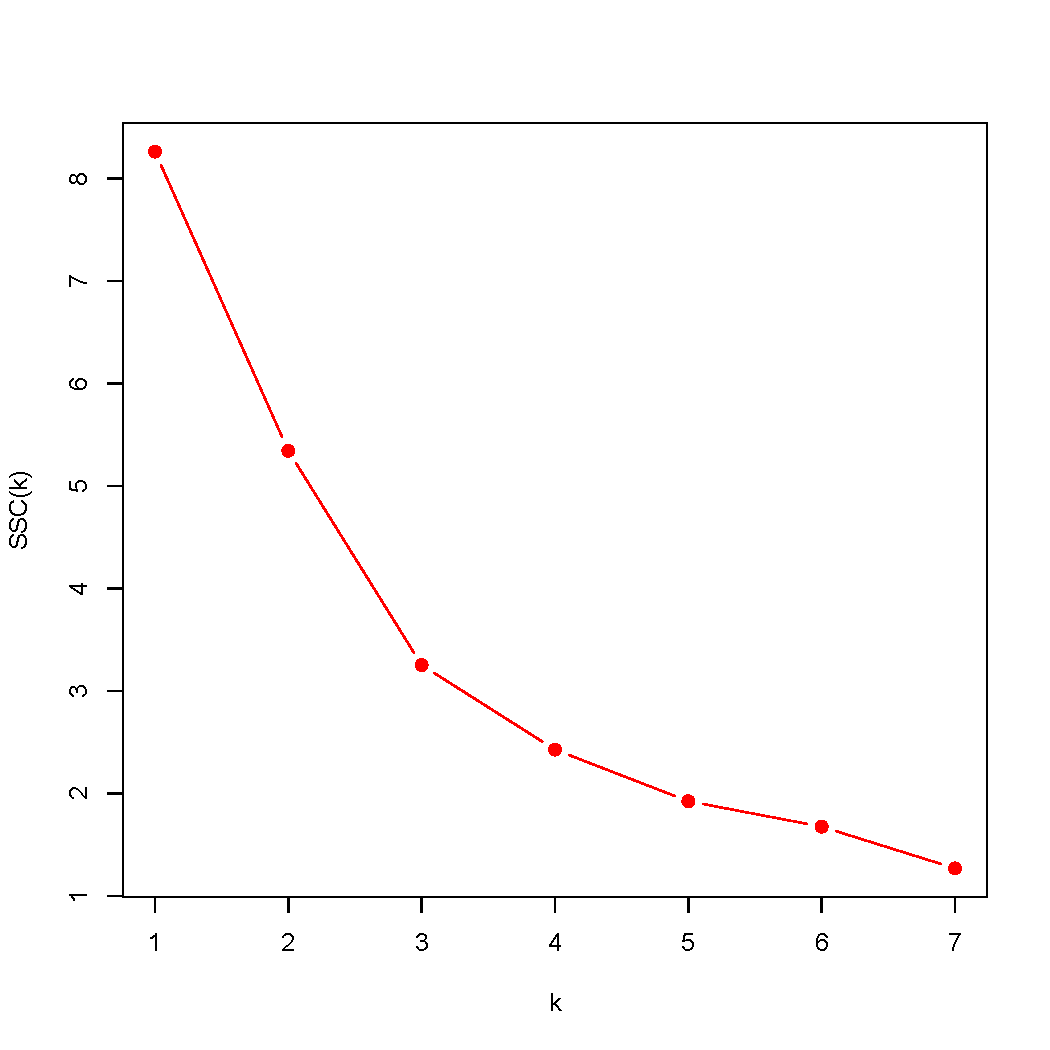
\includegraphics[width=0.58 \linewidth]{kink.pdf}\\[-1.5ex]
$k=3$ és el recomanable
\end{center}

\end{frame}

\begin{frame}
\frametitle{Quina $k$? Test F}
\vspace*{-2ex}

Es calcula
$$
F_k=\frac{SS_C(k)-SS_C(k+1)}{\frac{SS_C(k+1)}{p-k-1}}
$$
Es pren com a p-valor
$$
P(F_{n,n(p-k-1)}>F_k)
$$
amb $F_{n,n(p-k-1)}$ una F de Fisher amb $n$  i $n(p-k-1)$ graus de llibertat, i triam el $k$ amb p-valor més petit. 
\medskip

Cal dir que és un mètode molt emprat, però no massa justificable
\end{frame}


\begin{frame}
\frametitle{Quina $k$? Test F}

En l'exemple del gràfic anterior
\begin{center}
\footnotesize 
\begin{tabular}{r|cccccccc}
\hline
$k$ & 2 & 3 & 4 & 5 & 6 & 7 & 8\\ \hline
$SS_C(k)$ & 8.264 & 5.344 & 3.254 & 2.428& 1.925& 1.677 & 1.27\\ \hline
$F_k$ & 8.2 & 9 & 4.42 & 3.14 & 1.63 & 3.2 & \\ \hline
p-valor &  0.0014 & 0.001 & 0.02  & 0.06  & 0.229 & 0.06\\ \hline
\end{tabular}
\end{center}
\medskip

$k=3$ torna a ser el més recomanable
\medskip

Si el conjunt de punts és molt gran, tots els $p$-valors són propers a 0 i aquest mètode no és útil.

\end{frame}



\begin{frame}[fragile]
\frametitle{$k$-means amb R}

La instrucció bàsica per executar un $k$-means amb R és 
\begin{center}
\texttt{kmeans(x,centres,iter.max=...)}
\end{center}
amb 
\begin{itemize}
\item \texttt{x}, una matriu amb els punts $\mathbf{x}_i$ com a fileres 

\item \texttt{centres}, una matriu amb els centres  $\mathbf{c}_i$ de partida com a fileres, o el nombre $k$

\item \texttt{iter.max} el nombre màxim d'iteracions
\end{itemize}
Aquesta instrucció no segueix exactament el nostre algoritme, si voleu que executi l'algoritme explicat hi heu d'entrar, a més, \verb?algorithm="Lloyd"?

\end{frame}

\begin{frame}[fragile]
\frametitle{$k$-means amb R}

%\begin{lstlisting}
\begin{verbatim}
> dades=matrix(c(0.8,1.3,0.8,1.8,1.0,0.9,1.1,
0.1,1.1,1.6,1.4,0.6,1.5,0.1,2,2.1,1.5,2.3,1.8,
1.8,2.3,0.5,0.3,2.2,1,2.5,2,0.5,2,1.5,2.5,1,
0.5,0.5,1,2), nrow=18,byrow=TRUE) 
> cent=matrix(c(0.5,0,0.5,1.5,0.5,3),
nrow=3,byrow=TRUE)
\end{verbatim}
%\end{lstlisting}


\end{frame}

\begin{frame}[fragile]
\frametitle{$k$-means amb R}

\begin{verbatim}
> kmeans(dades,cent,algorithm="Lloyd")
$k$-means clustering with 3 clusters of sizes 
8, 5, 5
Cluster means:
    [,1]  [,2]
1 1.5375 0.525
2 1.3000 1.600
3 1.1600 2.220
Clustering vector:
 [1] 2 2 1 1 2 1 1 3 3 2 1 3 3 1 2 1 1 3
Within cluster sum of squares by cluster:
[1] 4.03375 1.46000 1.76000
 (between_SS / total_SS =  57.9 %)
...
\end{verbatim}
\end{frame}


\begin{frame}[fragile]
\frametitle{$k$-means amb R}
Components de la \texttt{list} \texttt{kmeans}:

\begin{itemize}
\item \red{\texttt{cluster}}: assignacions d'elements a clusters
\begin{verbatim}
> km=kmeans(dades,cent,algorithm="Lloyd")
> km$cluster
 [1] 2 2 1 1 2 1 1 3 3 2 1 3 3 1 2 1 1 3
\end{verbatim}
\item \red{\texttt{centers}}: els centres dels clusters
\begin{verbatim}
> km$centers
    [,1]  [,2]
1 1.5375 0.525
2 1.3000 1.600
3 1.1600 2.220
\end{verbatim}
\end{itemize}
\end{frame}


\begin{frame}[fragile]
\frametitle{$k$-means amb R}
Components de la \texttt{list} \texttt{kmeans}:

\begin{itemize}
\item \red{\texttt{totss}}: suma dels quadrats de les distàncies dels punts al punt mig de tots aquests punts.
\begin{verbatim}
> km$totss  
[1] 17.20944
\end{verbatim}
\item \red{\texttt{withinss}}: vector de les sumes, per a cada cluster, dels quadrats de les distàncies dels seus punts al punt mig del seu cluster.
\begin{verbatim}
> km$withinss
[1] 4.03375 1.46000 1.76000
\end{verbatim}
\end{itemize}
\end{frame}

\begin{frame}[fragile]
\frametitle{$k$-means amb R}
Components de la \texttt{list} \texttt{kmeans}:

\begin{itemize}
\item \red{\texttt{tot.withinss}}: suma de \texttt{withinss}, $SS_C$
\begin{verbatim}
> km$tot.withinss  
[1] 7.25375
\end{verbatim}
\item \red{\texttt{betweenss}}: diferència  $\texttt{totss}-\texttt{tot.withinss}$. És la suma, ponderada pel nombre d'objectes del cluster corresponent, dels quadrats de les distàncies dels centres dels clusters al punt mig de tots els punts.
\begin{verbatim}
> km$betweenss   
[1] 9.955694
\end{verbatim}
\end{itemize}
\end{frame}

\begin{frame}[fragile]
\frametitle{$k$-means amb R}
Components de la \texttt{list} \texttt{kmeans}:

\begin{itemize}
\item Ens interessa \red{\texttt{betweenss}/\texttt{totss}}, que mesura la fracció de la variabilitat de les dades que expliquen els clusters. Com més gran millor.

Al resultat de \texttt{kmeans} és \red{\texttt{between\_{}SS / total\_{}SS}}
\begin{verbatim}
> km
...
 (between_SS / total_SS =  57.9 %)
...
> 9.955694/17.20944  #betweenss/totss
[1] 0.5785019
\end{verbatim}

\end{itemize}
\end{frame}





\begin{frame}[fragile]
\frametitle{$k$-means amb R}
\vspace*{-2ex}

 
\begin{verbatim}
> km.rand=kmeans(dades,3,algorithm="Lloyd")
> km.rand
$k$-means clustering with 3 clusters of sizes 
6, 5, 7
Cluster means:
       [,1]     [,2]
1 2.1000000 1.233333
2 1.1000000 0.440000
3 0.9285714 1.957143
Clustering vector:
 [1] 3 3 2 2 3 2 2 1 3 1 1 3 3 1 1 1 2 3
Within cluster sum of squares by cluster:
[1] 2.593333 1.092000 1.851429
 (between_SS / total_SS =  67.8 %)
> km.rand$tot.withinss
[1] 5.965111
\end{verbatim}
\end{frame}




\begin{frame}[fragile]
\frametitle{$k$-means amb R}
\vspace*{-2ex}

 
\begin{verbatim}
> km2=kmeans(dades,3)  #5a repeticio ;-) 
> km2
K-means clustering with 3 clusters of sizes
5, 4, 9
Cluster means:
      [,1]     [,2]
1 1.100000 0.440000
2 2.200000 0.875000
3 1.144444 1.955556
Clustering vector:
 [1] 3 3 1 1 3 1 1 3 3 3 2 3 3 2 2 2 1 3
Within cluster sum of squares by cluster:
[1] 1.092000 0.867500 3.384444
 (between_SS / total_SS =  68.9 %)
> km2$tot.withinss
[1] 5.343944
\end{verbatim}
\end{frame}





\begin{frame}[fragile]
\frametitle{$k$-means amb R}

\begin{verbatim}
> plot(dades,col=km$cluster,pch=19,
 main="El nostre")
\end{verbatim}
\vspace*{-3ex}

\begin{center}
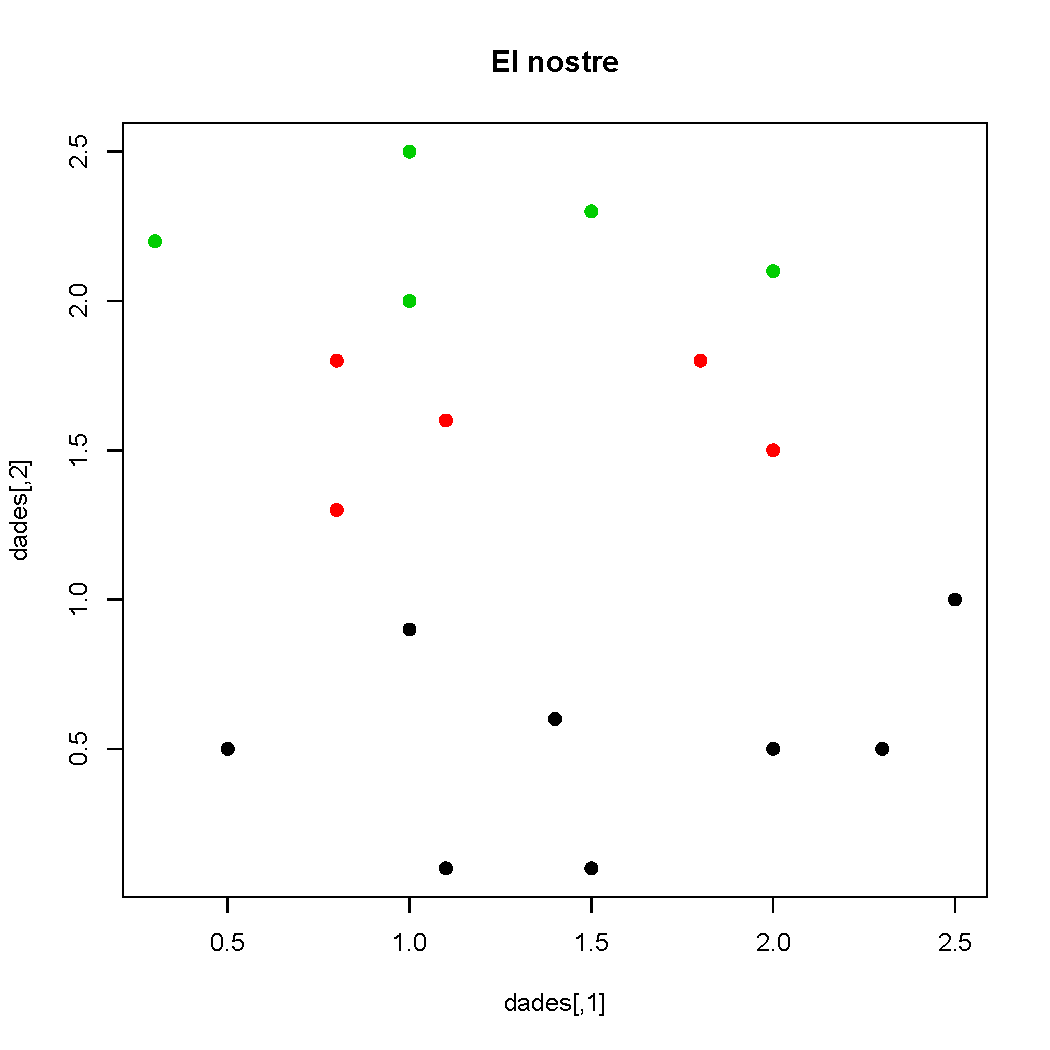
\includegraphics[width=0.7 \linewidth]{Rplot5.pdf}
\end{center}

\end{frame}

\begin{frame}[fragile]
\frametitle{$k$-means amb R}

\begin{verbatim}
> plot(dades,col=km2$cluster,pch=19,
 main="Optim")
\end{verbatim}
\vspace*{-3ex}

\begin{center}
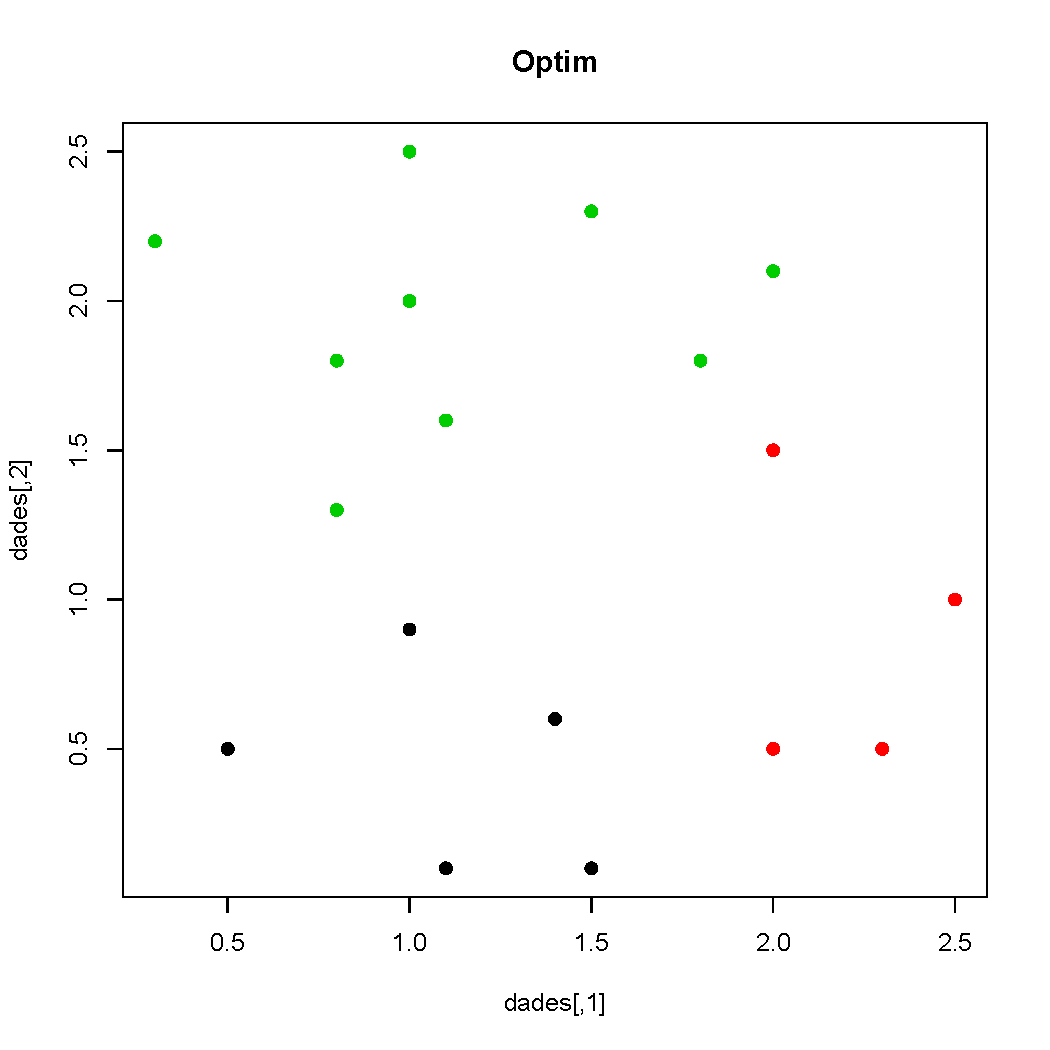
\includegraphics[width=0.7 \linewidth]{Rplot52.pdf}
\end{center}

\end{frame}


%
%\begin{frame}[fragile]
%\frametitle{$k$-means amb R}
% 
%\begin{verbatim}
%> library(cluster)
%> clusplot(dades,km$cluster,color=TRUE,
% shade=TRUE,labels=2,lines=0)
%\end{verbatim}
%\vspace*{-3ex}
%
%\begin{center}
%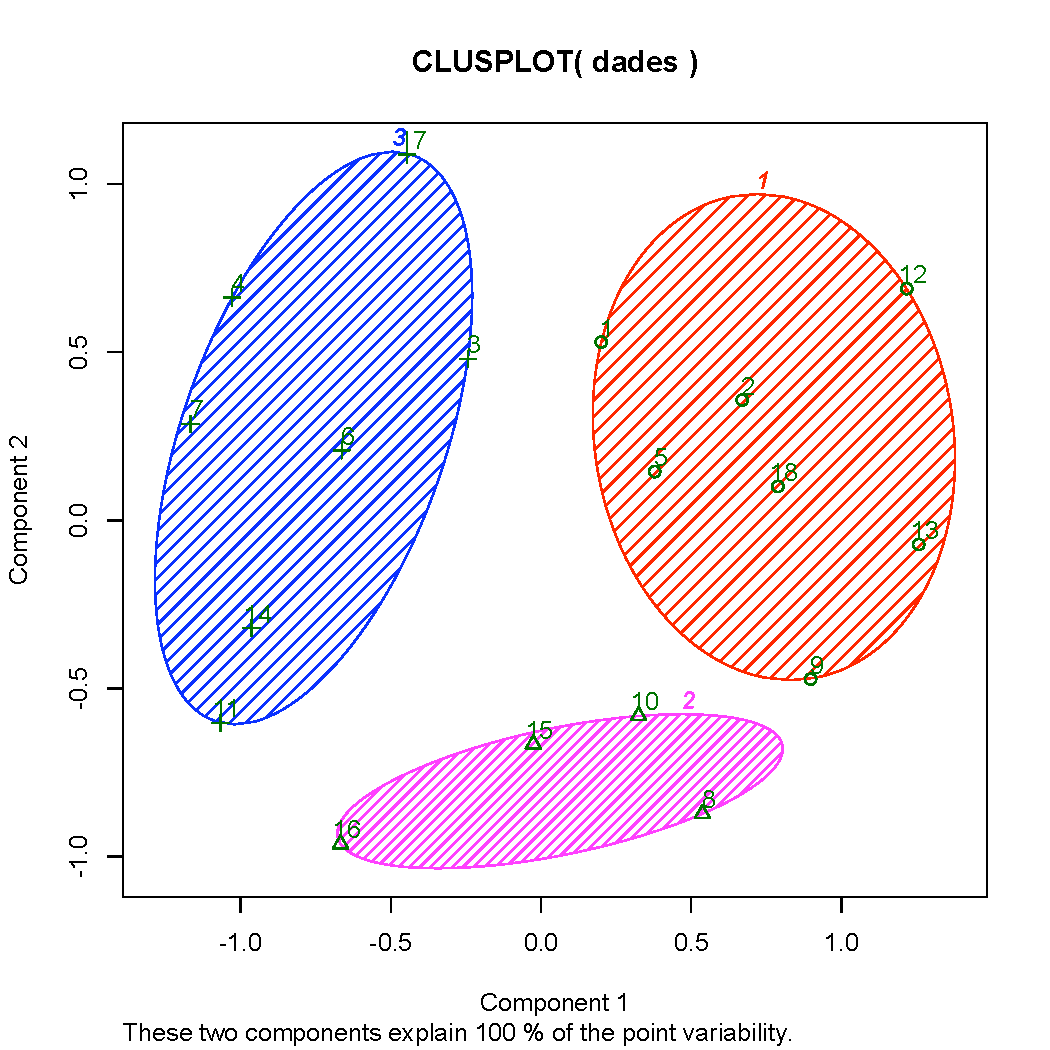
\includegraphics[width=0.7 \linewidth]{Rplot6.pdf}
%\end{center}
%
%\end{frame}


\subsection{Clustering jeràrquic}

\begin{frame}
\frametitle{Mètodes jeràrquics}

Els mètodes jeràrquics parteixen d'una matriu $D$ de semblances o de  distàncies entre els objectes
\medskip

Si tenim $p$ objectes, necessitam una matriu
$$
D=\left(\begin{array}{cccc}
d_{11} & d_{12} & \ldots & d_{1p}\\
d_{21} & d_{22} & \ldots & d_{2p}\\
\vdots & \vdots & \ddots & \vdots\\
d_{p1} & d_{p2} & \ldots & d_{pp}
\end{array}
\right)
$$
on cada $d_{ij}$ és la distància o la semblança entre l'objecte $i$ i l'objecte $j$
\end{frame}




\begin{frame}
\frametitle{Semblances}

Una \emph{semblança} sobre un conjunt $X$ és una aplicació $\sigma:X\times X\to [0,1]$ que és:
\begin{itemize}
\item \emph{Reflexiva}: Si $x=y$, aleshores $\sigma(x,y)=1$
\medskip

\item \emph{Simètrica}: $\sigma(x,y)=\sigma(y,x)$
\end{itemize}
\medskip

Dos objectes $x,y$ són més semblants com més gran és $\sigma(x,y)$
\end{frame}



\begin{frame}
\frametitle{Distàncies}

Una \emph{distància} sobre un conjunt $X$ és una aplicació $d:X\times X\to [0,\infty[$ que satisfà:
\begin{itemize}
\item \emph{Separació}: $d(x,y)=0$ si, i només si, $x=y$
\medskip

\item \emph{Simetria}: $d(x,y)=d(y,x)$
\medskip

\item \emph{Desigualtat triangular}: $d(x,z)\leq d(x,y)+d(y,z)$
\end{itemize}
\medskip

Dos objectes $x,y$ són més semblants com més petita és $d(x,y)$
\pause\bigskip


El primer problema és escollir la semblança o la distància a emprar, segons el significat que vulguem que tingui el clustering. \emph{És una decisió molt  important!}
\end{frame}

\begin{frame}
\frametitle{Dades binàries}
Partim de $p$ objectes, dels quals hem pres $n$ medicions, i els organitzam en fileres d'una matriu
$$
\mathbf{X}=
\begin{pmatrix}
x_{11}&x_{12}&\ldots&x_{1n} \\ 
x_{21}&x_{22}&\ldots&x_{2n} \\
\vdots&\vdots&\ddots&\vdots \\
x_{p1}&x_{p2}&\ldots&x_{pn}
\end{pmatrix}
$$

Suposem que les medicions són \emph{binàries} (0 o 1)\medskip

\blue{Exemple}:  Propietats dicotòmiques  d'organismes
\begin{center}
  \begin{tabular}{l|cccc}
& Pèl & Pulmons & Ovípar & Llet \\
\hline
Ca & 1 & 1 & 0 & 1\\
Granot & 0 & 1 & 1 & 0\\
Puput & 0 & 1 & 1 &0\\
Ornitorrinc & 1 & 1 & 1 & 1\\
Salmó & 0 & 0 & 1 & 0\\
\end{tabular}
\end{center}

\end{frame}

\begin{frame}
\frametitle{Dades binàries}
Donades dues fileres (objectes)
$$
\mathbf{x}_i=(x_{i1},\ldots,x_{in}),\quad \mathbf{x}_j=(x_{j1},\ldots,x_{jn}),
$$
definim les quantitats següents:
$$
\begin{array}{l}
a_0 = \big|\{k\mid x_{ik}=x_{jk}=0\}\big|\\[1ex]
a_1 =\big|\{k\mid x_{ik}=x_{jk}=1\}\big| \\[1ex]
a_2 = \big|\{k\mid x_{ik}\neq x_{jk}\}\big| \\[1ex]
\end{array}
$$
Una semblança entre els objectes $i$ i $j$ es pot definir mitjançant la fórmula genèrica
$$
\red{\sigma_{ij}=\frac{a_1 + \delta a_0}{\alpha a_1 + \beta a_0 +\lambda a_2}}
$$
\end{frame}

\begin{frame}
\frametitle{Dades binàries}
Els paràmetres $\delta$ i $\lambda$ són factors que donen pes a característiques. Els més comuns:
\medskip
\begin{center}
 
\begin{tabular}{|l|r|r|r|r|c|}
\hline
Nom&$\delta$&$\lambda$& $\alpha$ & $\beta$ & Definició\\\hline
Hamming&$1$&$1$&1 & 1& $\dfrac{a_1 + a_0}{n}$\vphantom{$\displaystyle\int_A^A$}\\\hline
Jaccard&$0$&$1$& 1&0 & $\dfrac{a_1}{a_1 + a_2}$ \vphantom{$\displaystyle\int_A^A$}\\\hline
Tanimoto&$1$&$2$&1 &1 & $\dfrac{a_1+a_0}{a_1+2a_2+a_0}$\vphantom{$\displaystyle\int_A^A$}\\\hline
Rusell--Rao&0 &1& 1& 1& $\dfrac{a_1}{n}$\vphantom{$\displaystyle\int_A^A$}\\\hline
Diu&$0$&$0.5$& 1& 0& $\dfrac{2a_1}{2a_1 + a_2}$\vphantom{$\displaystyle\int_A^A$} \\\hline
Kulczynski&0&1& 0& 0& $\dfrac{a_1}{a_2}$\vphantom{$\displaystyle\int_A^A$}\\\hline
\end{tabular}
\end{center}
\end{frame}


\begin{frame}
\frametitle{Exemple}
De 3 organismes hem observat si contenen o no gens homòlegs a 8 gens prototipus. Els resultats són els de la taula següent (1=Sí, 0=No)
\begin{center}
\begin{tabular}{c|cccccccc}
\multicolumn{1}{c}{} & \multicolumn{8}{c}{Gens}\\
Organisme & A & B & C & D & E & F & G & H\\ \hline
   X &                     0 & 1 & 1 & 0 & 1 & 1 & 0 & 0 \\
Y & 1 & 0 & 0 & 1 & 0 & 0 & 1 & 1 \\
Z & 0 & 0 & 1 & 0 & 1 & 0 & 1 & 0\\
\end{tabular}
\end{center}
\medskip

La matriu de semblances de Hamming és
$$
\mathbf{D}_{H}=
\begin{pmatrix}
1.000 & 0.000 & 0.625 \\
&1.000 & 0.375 \\
&&1.000
\end{pmatrix}
$$
\end{frame}


\begin{frame}
\frametitle{Matrius de contingència}
\vspace*{-3ex}

$$
\mathbf{X}=
\begin{pmatrix}
x_{11}&x_{12}&\ldots&x_{1n} \\ 
x_{21}&x_{22}&\ldots&x_{2n} \\
\vdots&\vdots&\ddots&\vdots \\
x_{p1}&x_{p2}&\ldots&x_{pn}
\end{pmatrix}
$$
on cada entrada és una freqüència
\medskip

Siguin
$$
x_{i\bullet}=\sum_{k=1}^n x_{ik},\
x_{\bullet k}=\sum_{i=1}^p x_{ik},\
x_{\bullet\bullet}=\sum_{i=1}^p  x_{i\bullet} = \sum_{k=1}^n x_{\bullet k}
$$
Se recomana prendre com a distància
$$
d_{ij}=\sqrt{\sum_{k=1}^n \frac{x_{\bullet\bullet}}{x_{\bullet k}} \left(\frac{x_{ik}}{x_{i\bullet}} - \frac{x_{jk}}{x_{j\bullet}}\right)^2}
$$

\end{frame}

\begin{frame}
\frametitle{Exemple}
\vspace*{-3ex}

A 3 boscos s'hi ha escollit una àrea de la mateixa superfície i s'hi han comptat els nombres d'exemplars de 5 plantes.
\begin{center}
\begin{tabular}{c|ccccc}
\multicolumn{1}{c}{} & \multicolumn{5}{c}{Planta}\\
Bosc & A & B & C & D & E \\ \hline
X & 12 & 3 & 8 & 0 & 24   \\
Y & 3 & 22 & 15 & 8 & 11   \\
Z & 0 & 7 & 12 & 20 & 6  \\
\end{tabular}
\end{center}
Taula amb freqüències marginals:
\begin{center}
\begin{tabular}{c|ccccc|c}
\multicolumn{1}{c}{} & \multicolumn{5}{c}{Planta} & \\
Bosc & A & B & C & D & E & $x_{i\bullet}$ \\ \hline
X & 12 & 3 & 8 & 0 & 24 & 47  \\
Y & 3 & 22 & 15 & 8 & 11  &  59  \\
Z & 0 & 7 & 12 & 20 & 6 & 45 \\\hline
$x_{\bullet j}$ & 15 & 32 & 35 & 28 & 41 & 151\\ \hline 
\end{tabular}
\end{center}




\end{frame}


\begin{frame}
\frametitle{Exemple}
\vspace*{-3ex}

\begin{center}
\begin{tabular}{c|ccccc|c}
\multicolumn{1}{c}{} & \multicolumn{5}{c}{Planta} & \\
Bosc & A & B & C & D & E & $x_{i\bullet}$ \\ \hline
X & 12 & 3 & 8 & 0 & 24 & 47  \\
Y & 3 & 22 & 15 & 8 & 11  &  59  \\
Z & 0 & 7 & 12 & 20 & 6 & 45 \\\hline
$x_{\bullet j}$ & 15 & 32 & 35 & 28 & 41 & 151\\ \hline 
\end{tabular}
\end{center}

$$
\begin{array}{rl}
d_{XY}^2 &\displaystyle =\frac{151}{15}\Big(\frac{12}{47}-\frac{3}{59}\Big)^2+
\frac{151}{32}\Big(\frac{3}{47}-\frac{22}{59}\Big)^2\\[2ex]
&\displaystyle \qquad +
\frac{151}{35}\Big(\frac{8}{47}-\frac{15}{59}\Big)^2+
\frac{151}{28}\Big(\frac{0}{47}-\frac{8}{59}\Big)^2\\[2ex]
&\displaystyle \qquad +
\frac{151}{41}\Big(\frac{24}{47}-\frac{11}{59}\Big)^2=\ldots
\end{array}
$$

\end{frame}


\begin{frame}
\frametitle{Exemple}
\vspace*{-3ex}

\begin{center}
\begin{tabular}{c|ccccc|c}
\multicolumn{1}{c}{} & \multicolumn{5}{c}{Planta} & \\
Bosc & A & B & C & D & E & $x_{i\bullet}$ \\ \hline
X & 12 & 3 & 8 & 0 & 24 & 47  \\
Y & 3 & 22 & 15 & 8 & 11  &  59  \\
Z & 0 & 7 & 12 & 20 & 6 & 45 \\\hline
$x_{\bullet j}$ & 15 & 32 & 35 & 28 & 41 & 151\\ \hline 
\end{tabular}
\end{center}
\medskip

$$
D=\left(\begin{array}{ccc}
0 & 1.178 & 1.525 \\
 & 0 & 0.880\\
 & & 0
 \end{array}\right) 
$$

\end{frame}




\begin{frame}
\frametitle{Dades contínues}
Quan tenim els objectes descrits com a vectors de $\RR^n$ i cada entrada correspon a l'observació d'una variable contínua, se solen emprar \emph{distàncies} basades en les \emph{normes $L_r$}: Donats
$$
\mathbf{x}_i=(x_{i1},\ldots,x_{in}),\quad \mathbf{x}_j=(x_{j1},\ldots,x_{jn}),
$$
la \emph{distància $L_r$} entre aquests és
$$
d_{ij}=\|\mathbf{x_i} - \mathbf{x_j}\|_r = \Big(\sum_{k=1}^n |x_{ik} - x_{jk}|^r\Big)^{1/r}
$$
\end{frame}


\begin{frame}
\frametitle{Dades contínues}
Quan $r=1$,
$$
d_{ij}= \sum_{k=1}^n |x_{ik} - x_{jk}|
$$
se'n diu la \emph{distància de Manhattan}
\medskip

Quan $r=2$,
$$
d_{ij}= \sqrt{\sum_{k=1}^n (x_{ik} - x_{jk})^2}
$$
és la \emph{distància euclidiana}
\end{frame}

\begin{frame}
\frametitle{Escalat de les dades}
De vegades és convenient que les dades estiguin en la mateixa escala, per evitar diferències en les contribucions de les diferents columnes 
\medskip

Quan s'empra la distància euclidiana, per escalar es divideix cada entrada $x_{ik}$ per la desviació típica $s_{\bullet k}$ de la  columna corresponent abans d'aplicar la distància.
\medskip

Queda
$$
d_{ij}= \sqrt{\sum_{k=1}^n \frac{(x_{ik} - x_{jk})^2}{s^2_{\bullet k}}}
$$
\end{frame}

\begin{frame}
\frametitle{Clustering jeràrquic}

Existeixen dos tipus de mètodes de clustering jeràrquic: 
\begin{itemize}
\item Els \emph{algoritmes aglomeratius} comencen amb la partició més fina possible (cada objecte constitueix un cluster) i els van agrupant.
\medskip

\item Els \emph{algoritmes de divisió} comencen amb la partició més grollera possible (tots els objectes constitueixen un cluster) i van dividint els clusters en clusters més petits.
\end{itemize}
\medskip

Els algoritmes aglomeratius són més populars, perquè en general requereixen menys temps de càlcul
\end{frame}



\subsection{Clustering jeràrquic aglomeratiu}
\begin{frame}
\frametitle{Algoritme bàsic de clustering jeràrquic aglomeratiu}
Algoritme bàsic 

\begin{enumerate}
\item Partim de $p$ objectes, i de la matriu $p\times p$ de \emph{distàncies} entre ells
\item Formam un cluster amb cada objecte
\item Trobam dos clusters a distància mínima $C_1$ i $C_2$
\item Unim $C_1$ i $C_2$ en un cluster nou $C_1+C_2$
\item Eliminam $C_1$ i $C_2$ de la llista de clusters
\item \emph{Recalculam la distància de $C_1+C_2$ als altres clusters}
\item Repetim (3)--(6) fins que només queda un únic cluster
\end{enumerate}


\end{frame}

\begin{frame}
\frametitle{Clustering jeràrquic aglomeratiu}
El càlcul de la distància entre clusters es pot fer de diverses maneres, donant lloc a resultats diferents:
\begin{itemize}
\item Per \emph{enllaç simple}: $d(C,C')=\min\{d(a,b)\mid a\in C,b\in C'\}$
\medskip

En aquest cas
$$
d(C,C_1+ C_2)=\min\{d(C,C_1),d(C,C_2)\}
$$

\item Per \emph{enllaç complet}: $d(C,C')=\max\{d(a,b)\mid a\in C,b\in C'\}$
\medskip

En aquest cas
$$d(C,C_1+ C_2)=\max\{d(C,C_1),d(C,C_2)\}$$
\end{itemize}


\end{frame}

\begin{frame}
\frametitle{Clustering jeràrquic aglomeratiu}
El càlcul de la distància entre clusters es pot fer de diverses maneres, donant lloc a resultats diferents:
\begin{itemize}

\item Per enllaç \emph{mitjà}: 
$$
d(C,C')=\displaystyle\frac{\sum_{a\in C, b\in C'} d(a,b)}{|C|\cdot |C'|}
$$

En aquest cas,
$$
\begin{array}{l}
d(C,C_1+ C_2)\\ \quad =\displaystyle \frac{|C_1|}{|C_1|+|C_2|}d(C,C_1)+\frac{|C_2|}{|C_1|+|C_2|}d(C,C_2)
\end{array}
$$

\item \ldots
\end{itemize}


\end{frame}

\begin{frame}
\frametitle{Clustering jeràrquic aglomeratiu}

En general, conegudes
$$
d(C,C_1),\quad d(C,C_2),\quad d(C_1,C_2),
$$
 hi ha una fórmula genèrica per calcular
$d(C,C_1+ C_2)$:
$$
\begin{array}{rl}
d(C,C_1+C_2)= &\hspace*{-1ex} \delta_1 d(C,C_1)+\delta_2 d(C,C_2)+\delta_3 d(C_1,C_2) \\[1ex] & + \delta_0 |d(C,C_1)-d(C,C_2)|,
\end{array}
$$
on els $\delta_i$ son paràmetres a triar.  Cada tria dóna un algoritme diferent, amb resultats possiblement diferents.

\end{frame}


\begin{frame}
\frametitle{Clustering jeràrquic aglomeratiu}
Si diem $n_X$ al nombre d'elements d'un cluster $X$:
\vskip 0.25cm

\begin{center}
\footnotesize \begin{tabular}{|l|@{}c|@{}c|@{}c|@{}c|}
\hline
Nom&$\delta_1$&$\delta_2$&$\delta_3$&$\delta_0$\\\hline
\red{Enllaç simple}\vphantom{$\displaystyle\int$} &$1/2$&$1/2$&$0$&$-1/2$\\\hline
\red{Enllaç complet}\vphantom{$\displaystyle\int$} &$1/2$&$1/2$&$0$&$1/2$\\\hline
\red{Enllaç mitjà}\vphantom{$\displaystyle\int_A^B$} &$\frac{n_{C_1}}{n_{C_1} + n_{C_2}}$&$\frac{n_{C_2}}{n_{C_1}+ n_{C_2}}$&$0$&$0$\\
\hline
Centroide\vphantom{$\displaystyle\int_A^B$} &$\frac{n_{C_1}}{n_{C_1} + n_{C_2}}$&$\frac{n_{C_2}}{n_{C_1} + n_{C_2}}$&$-\frac{n_{C_1} n_{C_2}}{(n_{C_1} + n_{C_2})^2}$&$0$\\\hline
Mediana\vphantom{$\displaystyle\int_A^B$} &$1/2$&$1/2$&$-1/4$&$0$\\\hline
\emph{Ward}\vphantom{$\displaystyle\int_A^B$} &$\frac{n_{C} + n_{C_1}}{n_C + n_{C_1} + n_{C_2}}$&$\frac{n_C + n_{C_2}}{n_C + n_{C_1}+ n_{C_2}}$&$-\frac{n_C}{n_C + n_{C_1} + n_{C_2}}$&$0$\\\hline
\end{tabular}
\end{center}
\end{frame}





\begin{frame}
\frametitle{Exemple}
A,B,C,D,E,F,G: plantes; \\
x, y: gens; \\
dades:  expressió del gen en condicions de sequera
\vspace*{-2ex}

\begin{columns}[t]
\begin{column}{0.5\textwidth}
\begin{center}
\begin{tabular}{c|cc}
& x & y\\
\hline
A & 0.8 & 1.8\\
B & 1.1 & 1.6\\
C & 0.8 & 1.3\\
D & 1.0 & 0.9\\
E & 1.4 & 0.6\\
F & 1.5 & 0.1\\
G& 1.1 & 0.1
\end{tabular}
\end{center}
\end{column}
\begin{column}{0.5\textwidth}
\begin{center}
\begin{tikzpicture}[thick,>=stealth,scale=2]
\filldraw [black] (0.8, 1.3) circle (1pt); %C
\draw (0.7,1.3) node{\footnotesize C}; 
\filldraw [black] (0.8 , 1.8) circle (1pt); %A
\draw (0.7,1.8) node{\footnotesize A}; 
\filldraw [black] (1.0,0.9) circle (1pt); %D
\draw (0.9,0.9) node{\footnotesize D}; 
\filldraw [black] (1.1,0.1) circle (1pt); %G
\draw (1.0,0.1) node{\footnotesize G}; 
\filldraw [black] (1.1, 1.6) circle (1pt); %B
\draw (1.0,1.6) node{\footnotesize B}; 
\filldraw [black] (1.4, 0.6) circle (1pt); %E
\draw (1.3,0.6) node{\footnotesize E}; 
\filldraw [black] (1.5 ,0.1) circle (1pt); %F
\draw (1.4,0.1) node{\footnotesize F}; 
\draw (0,-0.2)--(0,2);
\draw (-0.2,0)--(2,0);
\draw (0.5,0)--(0.5,-0.1);
\draw (0.5,-0.2) node {\footnotesize 0.5};
\draw (1,0)--(1,-0.1);
\draw (1,-0.2) node {\footnotesize 1};
\draw (1.5,0)--(1.5,-0.1);
\draw (1.5,-0.2) node {\footnotesize 1.5};
\draw (-0.1,0.5)--(0,0.5);
\draw (-0.2,0.5) node {\footnotesize 0.5};
\draw (-0.1,1)--(0,1);
\draw (-0.2,1) node {\footnotesize 1};
\draw (-0.1,1.5)--(0,1.5);
\draw (-0.2,1.5) node {\footnotesize 1.5};

\end{tikzpicture}
\end{center}
\end{column}
\end{columns}
\medskip

Comparam les dades amb distància euclidiana. Emprarem enllaç simple.
\end{frame}


\begin{frame}
\frametitle{Exemple}
Matriu de distàncies
\begin{center}
\footnotesize \begin{tabular}{c|ccccccc}
& A & B & C & D & E & F & G \\
\hline
A & \\
B & 0.3606 \\
C & 0.5000 & 0.4243\\
D & 0.9220 & 0.7071 & 0.4472\\
E & 1.3416 & 1.0440 & 0.9220 & 0.5000 \\
F & 1.8385 & 1.5524 & 1.3892 & 0.9434 & 0.5099\\
G & 1.7263 & 1.5000 & 1.2369 & 0.8062 & 0.5381 & 0.4000\\
\end{tabular}
\end{center}

\end{frame}

\begin{frame}
\frametitle{Exemple}
Detectam un mínim
\begin{center}
\footnotesize \begin{tabular}{c|ccccccc}
& A & B & C & D & E & F & G \\
\hline
A & \\
B & \red{0.3606} \\
C & 0.5000 & 0.4243\\
D & 0.9220 & 0.7071 & 0.4472\\
E & 1.3416 & 1.0440 & 0.9220 & 0.5000 \\
F & 1.8385 & 1.5524 & 1.3892 & 0.9434 & 0.5099\\
G & 1.7263 & 1.5000 & 1.2369 & 0.8062 & 0.5381 & 0.4000\\
\end{tabular}
\end{center}

Substituïm \{A,B\} per H i recalculam
\begin{center}
\footnotesize \begin{tabular}{c|cccccc}
& H & C & D & E & F & G \\
\hline
H & \\
C & 0.4243\\
D & 0.7071 & 0.4472\\
E & 1.0440 & 0.9220 & 0.5000 \\
F & 1.5524 & 1.3892 & 0.9434 & 0.5099\\
G & 1.5000 & 1.2369 & 0.8062 & 0.5381 & 0.4000\\
\end{tabular}
\end{center}
\end{frame}

\begin{frame}
\frametitle{Exemple}
\vspace*{1ex}

\begin{center}
\begin{tikzpicture}[thick,>=stealth,scale=0.5]
\draw (0,0) node[tree] (A) {}; 
\draw (2,0) node[tree] (B) {};  
\draw (4,0) node[tree] (C) {};  
\draw (6,0) node[tree] (D) {};  
\draw (8,0) node[tree] (E) {};  
\draw (10,0) node[tree] (F) {};  
\draw (12,0) node[tree] (G) {};  
\draw (A.south) node[below] {$A$};
\draw (B.south) node[below] {$B$};
\draw (C.south) node[below] {$C$};
\draw (D.south) node[below] {$D$};
\draw (E.south) node[below] {$E$};
\draw (F.south) node[below] {$F$};
\draw (G.south) node[below] {$G$};
\draw (A)--(0,2)--(2,2)--(B);
\draw (1,2) node (H) {};
\draw (H.north) node[above] {$H$};
\draw (10,10) node {};
\end{tikzpicture}

\end{center}
\end{frame}



\begin{frame}
\frametitle{Exemple}
Detectam un mínim
\begin{center}
\footnotesize \begin{tabular}{c|cccccc}
& H & C & D & E & F & G \\
\hline
H & \\
C & 0.4243\\
D & 0.7071 & 0.4472\\
E & 1.0440 & 0.9220 & 0.5000 \\
F & 1.5524 & 1.3892 & 0.9434 & 0.5099\\
G & 1.5000 & 1.2369 & 0.8062 & 0.5381 & \red{0.4000}\\
\end{tabular}
\end{center}

Substituïm \{F,G\}  per I i recalculam
\begin{center}
\footnotesize \begin{tabular}{c|cccccc}
& H & C & D & E & I \\
\hline
H & \\
C & 0.4243\\
D & 0.7071 & 0.4472\\
E & 1.0440 & 0.9220 & 0.5000 \\
I & 1.5000 & 1.2369 & 0.8062 & 0.5099\\
\end{tabular}
\end{center}


\end{frame}

\begin{frame}
\frametitle{Exemple}
\vspace*{1ex}

\begin{center}
\begin{tikzpicture}[thick,>=stealth,scale=0.5]
\draw (0,0) node[tree] (A) {}; 
\draw (2,0) node[tree] (B) {};  
\draw (4,0) node[tree] (C) {};  
\draw (6,0) node[tree] (D) {};  
\draw (8,0) node[tree] (E) {};  
\draw (10,0) node[tree] (F) {};  
\draw (12,0) node[tree] (G) {};  
\draw (A.south) node[below] {$A$};
\draw (B.south) node[below] {$B$};
\draw (C.south) node[below] {$C$};
\draw (D.south) node[below] {$D$};
\draw (E.south) node[below] {$E$};
\draw (F.south) node[below] {$F$};
\draw (G.south) node[below] {$G$};
\draw (A)--(0,2)--(2,2)--(B);
\draw (F)--(10,2)--(12,2)--(G);
\draw (1,2) node (H) {};
\draw (H.north) node[above] {$H$};
\draw (11,2) node (I) {};
\draw (I.north) node[above] {$I$};
\draw (10,10) node {};
\end{tikzpicture}

\end{center}
\end{frame}


\begin{frame}
\frametitle{Exemple}
Detectam un mínim
\begin{center}
\footnotesize \begin{tabular}{c|cccccc}
& H & C & D & E & I \\
\hline
H & \\
C & \red{0.4243}\\
D & 0.7071 & 0.4472\\
E & 1.0440 & 0.9220 & 0.5000 \\
I & 1.5000 & 1.2369 & 0.8062 & 0.5099\\
\end{tabular}
\end{center}

Substituïm \{H,C\} per J i recalculam
\begin{center}
\footnotesize \begin{tabular}{c|ccccc}
& J & D & E & I \\
\hline
J & \\
D &  0.4472\\
E &   0.9220 & 0.5000 \\
I &   1.2369 & 0.8062 & 0.5099\\
\end{tabular}
\end{center}


\end{frame}

\begin{frame}
\frametitle{Exemple}
\vspace*{1ex}

\begin{center}
\begin{tikzpicture}[thick,>=stealth,scale=0.5]
\draw (0,0) node[tree] (A) {}; 
\draw (2,0) node[tree] (B) {};  
\draw (4,0) node[tree] (C) {};  
\draw (6,0) node[tree] (D) {};  
\draw (8,0) node[tree] (E) {};  
\draw (10,0) node[tree] (F) {};  
\draw (12,0) node[tree] (G) {};  
\draw (A.south) node[below] {$A$};
\draw (B.south) node[below] {$B$};
\draw (C.south) node[below] {$C$};
\draw (D.south) node[below] {$D$};
\draw (E.south) node[below] {$E$};
\draw (F.south) node[below] {$F$};
\draw (G.south) node[below] {$G$};
\draw (A)--(0,2)--(2,2)--(B);
\draw (F)--(10,2)--(12,2)--(G);
\draw (1,2)--(1,4)--(4,4)--(C);
\draw (1,2) node (H) {};
\draw (H.south) node[below] {$H$};
\draw (11,2) node (I) {};
\draw (I.north) node[above] {$I$};
\draw (2.5,4) node (J) {};
\draw (J.north) node[above] {$J$};
\draw (10,10) node {};
\end{tikzpicture}

\end{center}
\end{frame}

\begin{frame}
\frametitle{Exemple}
Detectam un mínim
\begin{center}
\footnotesize \begin{tabular}{c|ccccc}
& J & D & E & I \\
\hline
J & \\
D &  \red{0.4472}\\
E &   0.9220 & 0.5000 \\
I &   1.2369 & 0.8062 & 0.5099\\
\end{tabular}
\end{center}

Substituïm \{J,D\}  per K i recalculam
\begin{center}
\footnotesize \begin{tabular}{c|cccc}
& K & E & I \\
\hline
K & \\
E &    0.5000 \\
I &   0.8062 & 0.5099\\
\end{tabular}
\end{center}

\end{frame}

\begin{frame}
\frametitle{Exemple}
\vspace*{1ex}

\begin{center}
\begin{tikzpicture}[thick,>=stealth,scale=0.5]
\draw (0,0) node[tree] (A) {}; 
\draw (2,0) node[tree] (B) {};  
\draw (4,0) node[tree] (C) {};  
\draw (6,0) node[tree] (D) {};  
\draw (8,0) node[tree] (E) {};  
\draw (10,0) node[tree] (F) {};  
\draw (12,0) node[tree] (G) {};  
\draw (A.south) node[below] {$A$};
\draw (B.south) node[below] {$B$};
\draw (C.south) node[below] {$C$};
\draw (D.south) node[below] {$D$};
\draw (E.south) node[below] {$E$};
\draw (F.south) node[below] {$F$};
\draw (G.south) node[below] {$G$};
\draw (A)--(0,2)--(2,2)--(B);
\draw (F)--(10,2)--(12,2)--(G);
\draw (1,2)--(1,4)--(4,4)--(C);
\draw (2.5,4)--(2.5,6)--(6,6)--(D);
\draw (1,2) node (H) {};
\draw (H.south) node[below] {$H$};
\draw (11,2) node (I) {};
\draw (I.north) node[above] {$I$};
\draw (2.5,4) node (J) {};
\draw (J.south) node[below] {$J$};
\draw (4.25,6) node (K) {};
\draw (K.north) node[above] {$K$};
\draw (10,10) node {};
\end{tikzpicture}

\end{center}
\end{frame}

\begin{frame}
\frametitle{Exemple}
Detectam un mínim
\begin{center}
\footnotesize \begin{tabular}{c|cccc}
& K & E & I \\
\hline
K & \\
E &    \red{0.5000} \\
I &   0.8062 & 0.5099\\
\end{tabular}
\end{center}

Substituïm \{K,E\} per L i recalculam
\begin{center}
\footnotesize \begin{tabular}{c|ccc}
& L & I \\
\hline
L & \\
I &   0.5099\\
\end{tabular}
\end{center}


\end{frame}

\begin{frame}
\frametitle{Exemple}
\vspace*{1ex}

\begin{center}
\begin{tikzpicture}[thick,>=stealth,scale=0.5]
\draw (0,0) node[tree] (A) {}; 
\draw (2,0) node[tree] (B) {};  
\draw (4,0) node[tree] (C) {};  
\draw (6,0) node[tree] (D) {};  
\draw (8,0) node[tree] (E) {};  
\draw (10,0) node[tree] (F) {};  
\draw (12,0) node[tree] (G) {};  
\draw (A.south) node[below] {$A$};
\draw (B.south) node[below] {$B$};
\draw (C.south) node[below] {$C$};
\draw (D.south) node[below] {$D$};
\draw (E.south) node[below] {$E$};
\draw (F.south) node[below] {$F$};
\draw (G.south) node[below] {$G$};
\draw (A)--(0,2)--(2,2)--(B);
\draw (F)--(10,2)--(12,2)--(G);
\draw (1,2)--(1,4)--(4,4)--(C);
\draw (2.5,4)--(2.5,6)--(6,6)--(D);
\draw (4.25,6)--(4.25,8)--(8,8)--(E);
\draw (1,2) node (H) {};
\draw (H.south) node[below] {$H$};
\draw (11,2) node (I) {};
\draw (I.north) node[above] {$I$};
\draw (2.5,4) node (J) {};
\draw (J.south) node[below] {$J$};
\draw (4.25,6) node (K) {};
\draw (K.south) node[below] {$K$};
\draw (6.37,8) node (L) {};
\draw (L.north) node[above] {$L$};
\draw (10,10) node {};
\end{tikzpicture}

\end{center}
\end{frame}


\begin{frame}
\frametitle{Exemple}
Finalment, unim L i I en un sol cluster

\begin{center}
\begin{tikzpicture}[thick,>=stealth,scale=0.5]
\draw (0,0) node[tree] (A) {}; 
\draw (2,0) node[tree] (B) {};  
\draw (4,0) node[tree] (C) {};  
\draw (6,0) node[tree] (D) {};  
\draw (8,0) node[tree] (E) {};  
\draw (10,0) node[tree] (F) {};  
\draw (12,0) node[tree] (G) {};  
\draw (A.south) node[below] {$A$};
\draw (B.south) node[below] {$B$};
\draw (C.south) node[below] {$C$};
\draw (D.south) node[below] {$D$};
\draw (E.south) node[below] {$E$};
\draw (F.south) node[below] {$F$};
\draw (G.south) node[below] {$G$};
\draw (A)--(0,2)--(2,2)--(B);
\draw (F)--(10,2)--(12,2)--(G);
\draw (1,2)--(1,4)--(4,4)--(C);
\draw (2.5,4)--(2.5,6)--(6,6)--(D);
\draw (4.25,6)--(4.25,8)--(8,8)--(E);
\draw (6.37,8)--(6.37,10)--(11,10)--(11,2);
\draw (10,10) node {};
\end{tikzpicture}

\end{center}
\end{frame}

\begin{frame}
\frametitle{Limitacions del clustering jeràrquic aglomeratiu}
\begin{itemize}
\item La distància que s'hi empra és molt important
\medskip

\item No hi ha teoria que avali quin mètode per calcular la distància entre clusters és el millor en cada cas
\medskip

\item Realment, no defineix directament clusters, però tallant en una alçada del dendrograma n'obtenim
\medskip

\item Sempre agrupa de dos en dos, i de vegades pren decisions aleatòries per aconseguir-ho

\end{itemize}
\end{frame}

\begin{frame}[fragile]
\frametitle{Clustering jeràrquic aglomeratiu amb R}

La  instrucció bàsica és
\begin{center}
\verb?hclust(d, method = "...")?
\end{center}
on
\begin{itemize}
\item \texttt{d} és una matriu de distàncies
\medskip

\item \texttt{method} serveix per especificar el mètode:  \verb?"single"?,  \verb?"complete"?, \verb?"average"?, \verb?"ward"?, \verb?"median"?,  \verb?"centroid"?, \ldots
\end{itemize}
\end{frame}



\begin{frame}[fragile]
\frametitle{Clustering jeràrquic aglomeratiu amb R}

Per representar el clustering per mitjà d'un dendrograma, cal aplicar al resultat de \texttt{hclust} la instrucció
\begin{center}
\verb?plot(clust, labels=..., hang=..., ...)?
\end{center}
on
\begin{itemize}
\item \texttt{clust} és un \texttt{hclust}
\medskip

\item \texttt{labels} serveix per posar noms als objectes
\medskip

\item \texttt{hang} serveix per especificar la posició de les etiquetes: mirau el \texttt{help}

\item Altres paràmetres usuals dels \texttt{plot}
\end{itemize}

\end{frame}



\begin{frame}[fragile]
\frametitle{Clustering jeràrquic aglomeratiu amb R}


Per calcular la distància entre les fileres d'una matriu, podem emprar
\begin{center}
\verb?dist(x, method = "...")?
\end{center}
on
\begin{itemize}
\item \texttt{x} és una matriu de dades
\medskip

\item \texttt{method} serveix per especificar el mètode:   \verb?"euclidean"?,  \verb?"manhattan"?, \ldots
\end{itemize}
\medskip
\end{frame}



\begin{frame}[fragile]
\frametitle{Exemple}

\begin{verbatim}
> dades=matrix(data=c(0.8,1.8,1.1,1.6, 0.8,1.3,
  1.0,0.9,1.4, 0.6,1.5, 0.1,1.1,0.1), 
  nrow=7,byrow=TRUE)
> dades
     [,1] [,2]
[1,]  0.8  1.8
[2,]  1.1  1.6
[3,]  0.8  1.3
[4,]  1.0  0.9
[5,]  1.4  0.6
[6,]  1.5  0.1
[7,]  1.1  0.1
\end{verbatim}


\end{frame}

\begin{frame}[fragile]
\frametitle{Exemple}

\begin{verbatim}
> distancies=dist(dades,method="euclidean")
> distancies
     1      2      3      4      5      6
2 0.3606                                                  
3 0.5000 0.4243                                        
4 0.9220 0.7071  0.4472                             
5 1.3417 1.0440  0.9220  0.5000                  
6 1.8385 1.5524  1.3892  0.9434  0.5099           
7 1.7263 1.5000  1.2370  0.8062  0.5831  0.4000 
\end{verbatim}
\end{frame}

\begin{frame}[fragile]
\frametitle{Exemple}

\begin{verbatim}
> clustering=hclust(distancies,method="single")
> clustering$merge #formació de clusters
     [,1] [,2]
[1,]   -1   -2
[2,]   -6   -7
[3,]   -3    1
[4,]   -4    3
[5,]   -5    4
[6,]    2    5
> clustering$height  #distàncies mínimes
[1] 0.3605551 0.4000000 0.4242641 0.4472136 
  0.5000000 0.5099020
\end{verbatim}





\end{frame}






\begin{frame}[fragile]
\frametitle{Exemple}

\begin{verbatim}
> especies=c("A","B","C","D","E","F","G")
> plot(clustering,labels=especies)
\end{verbatim}
\vspace*{-3ex}

\begin{center}
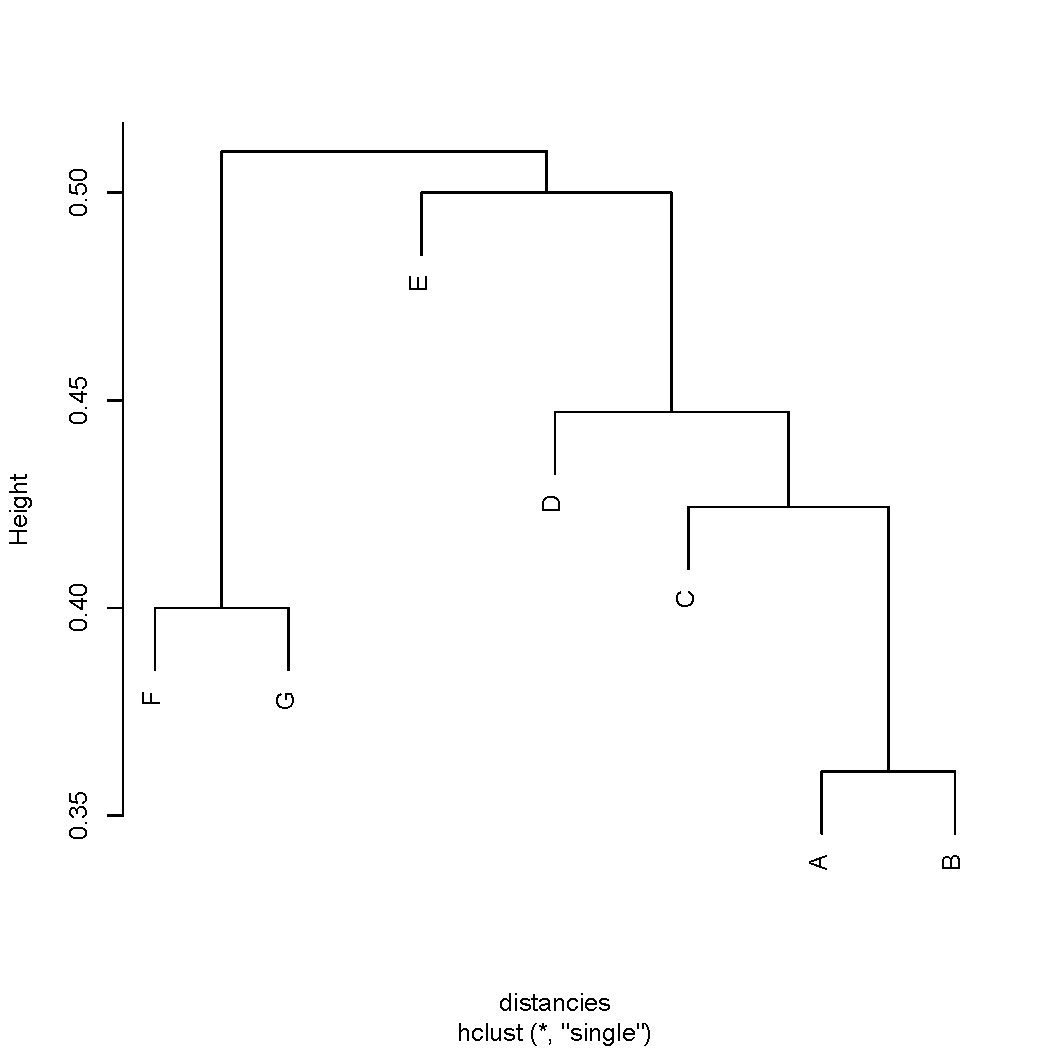
\includegraphics[width=0.7\linewidth]{Rplot1.pdf}
\end{center}
\end{frame}

\begin{frame}[fragile]
\frametitle{Clustering jeràrquic amb R}

\begin{verbatim}
> plot(hclust(distancies,method="single"),
 labels=especies,hang=-1)
\end{verbatim}
\begin{center}
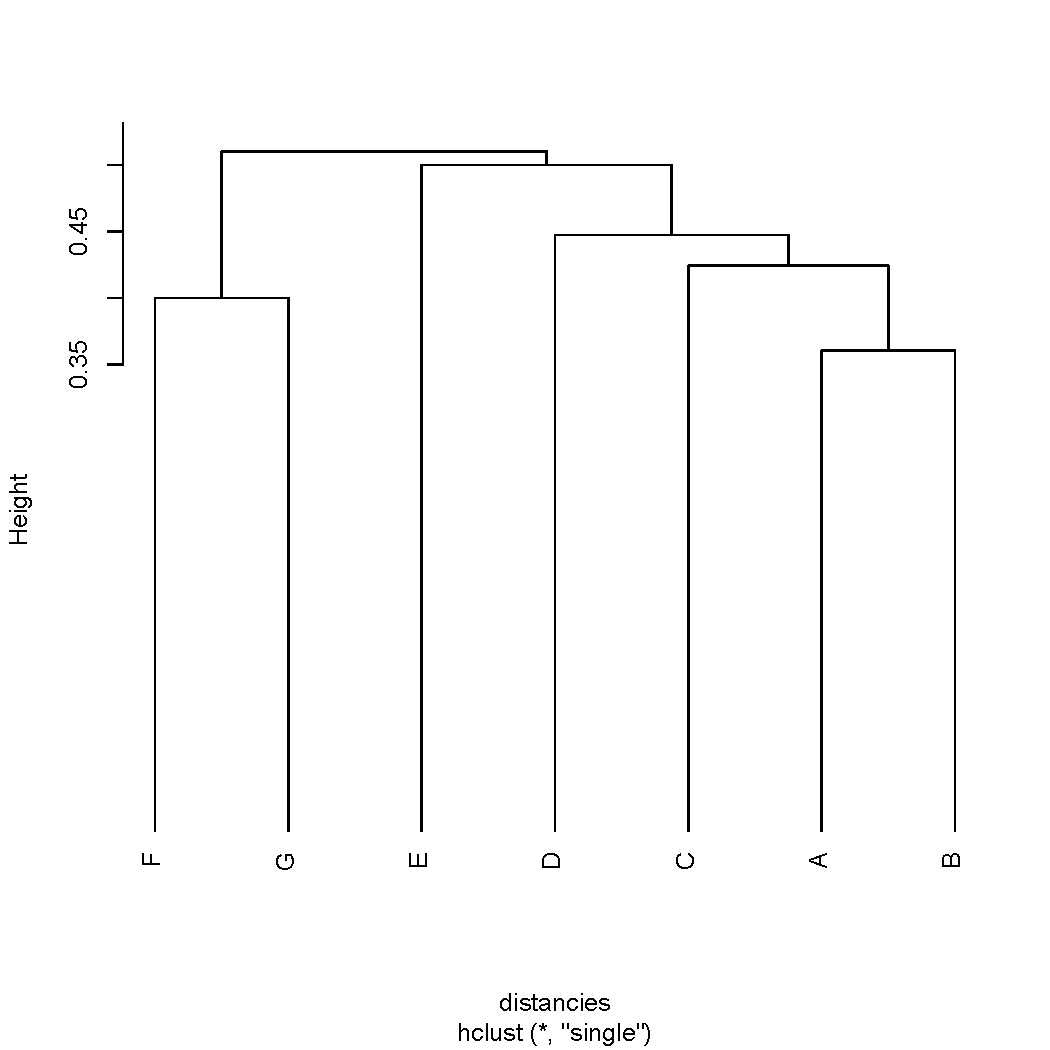
\includegraphics[width=0.7\linewidth]{Rplot2.pdf}
\end{center}
\end{frame}

\begin{frame}[fragile]
\frametitle{Clustering jeràrquic amb R}

\begin{verbatim}
> plot(hclust(distancies,method="average"),
 labels=especies,hang=-1)
\end{verbatim}
\begin{center}
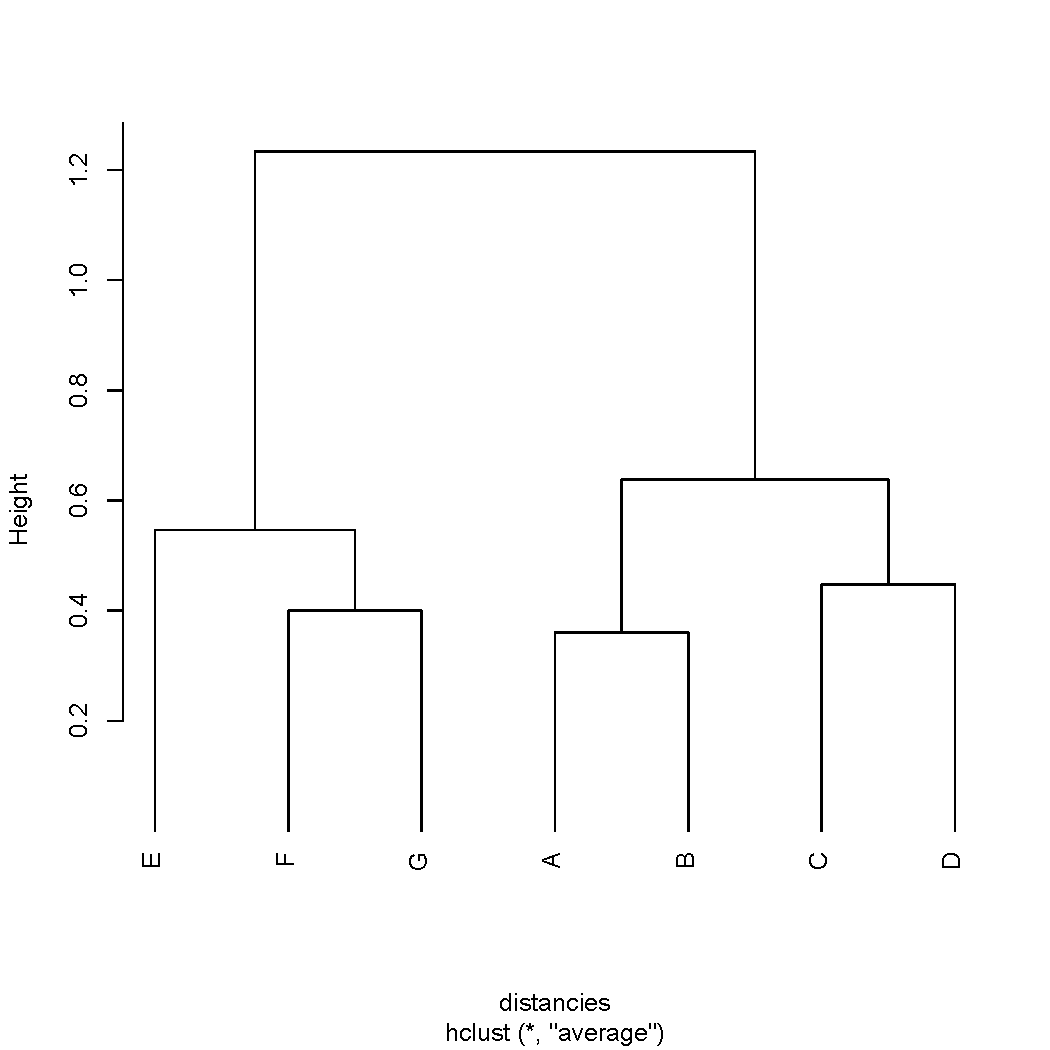
\includegraphics[width=0.7\linewidth]{Rplot3.pdf}
\end{center}
\end{frame}

\begin{frame}[fragile]
\frametitle{Clustering jeràrquic amb R}

\begin{verbatim}
> plot(hclust(distancies,method="complete"),
 labels=especies,hang=-1)
\end{verbatim}
\begin{center}
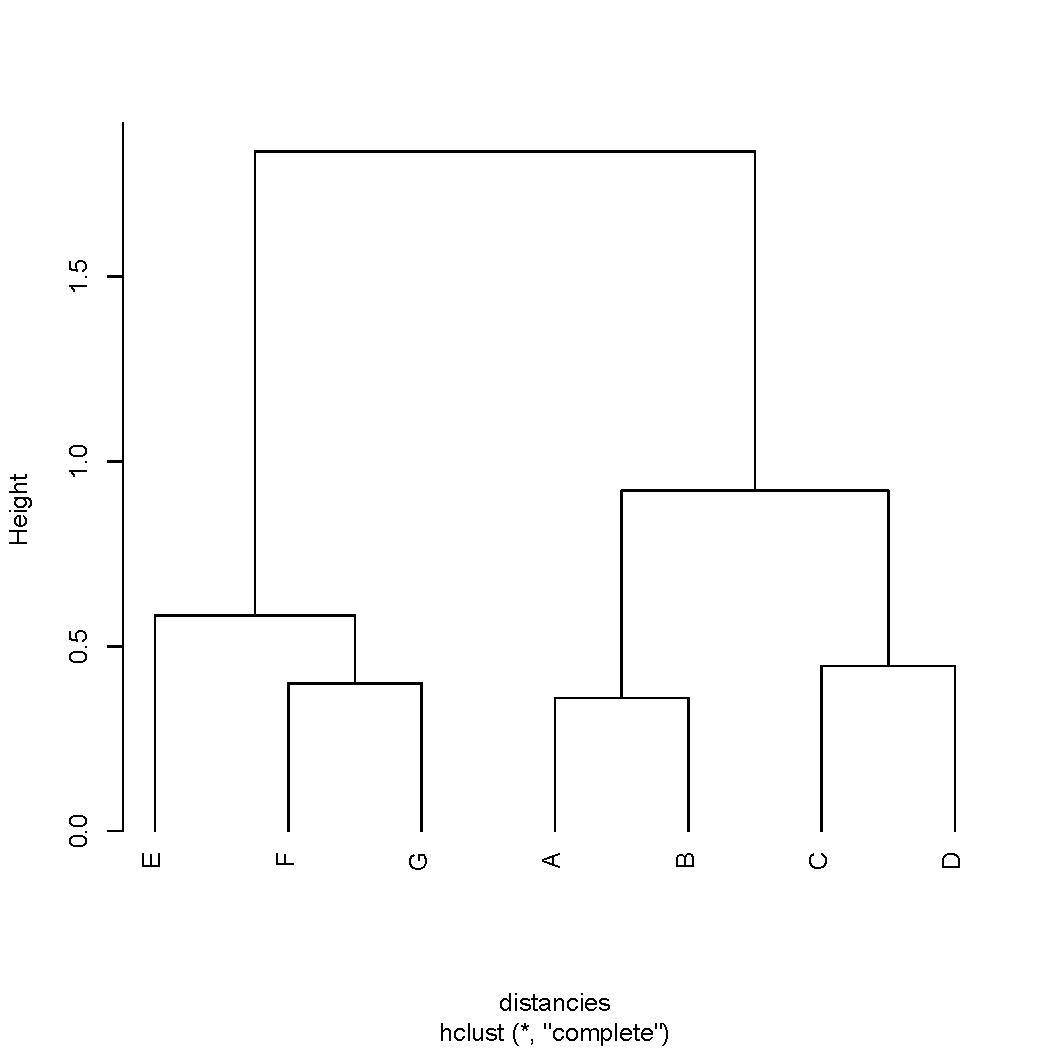
\includegraphics[width=0.7\linewidth]{Rplot4.pdf}
\end{center}
\end{frame}

\begin{frame}[fragile]
\frametitle{Clustering jeràrquic amb R}

\begin{verbatim}
> plot(hclust(distancies,method="ward"),
 labels=especies,hang=-1)
\end{verbatim}
\begin{center}
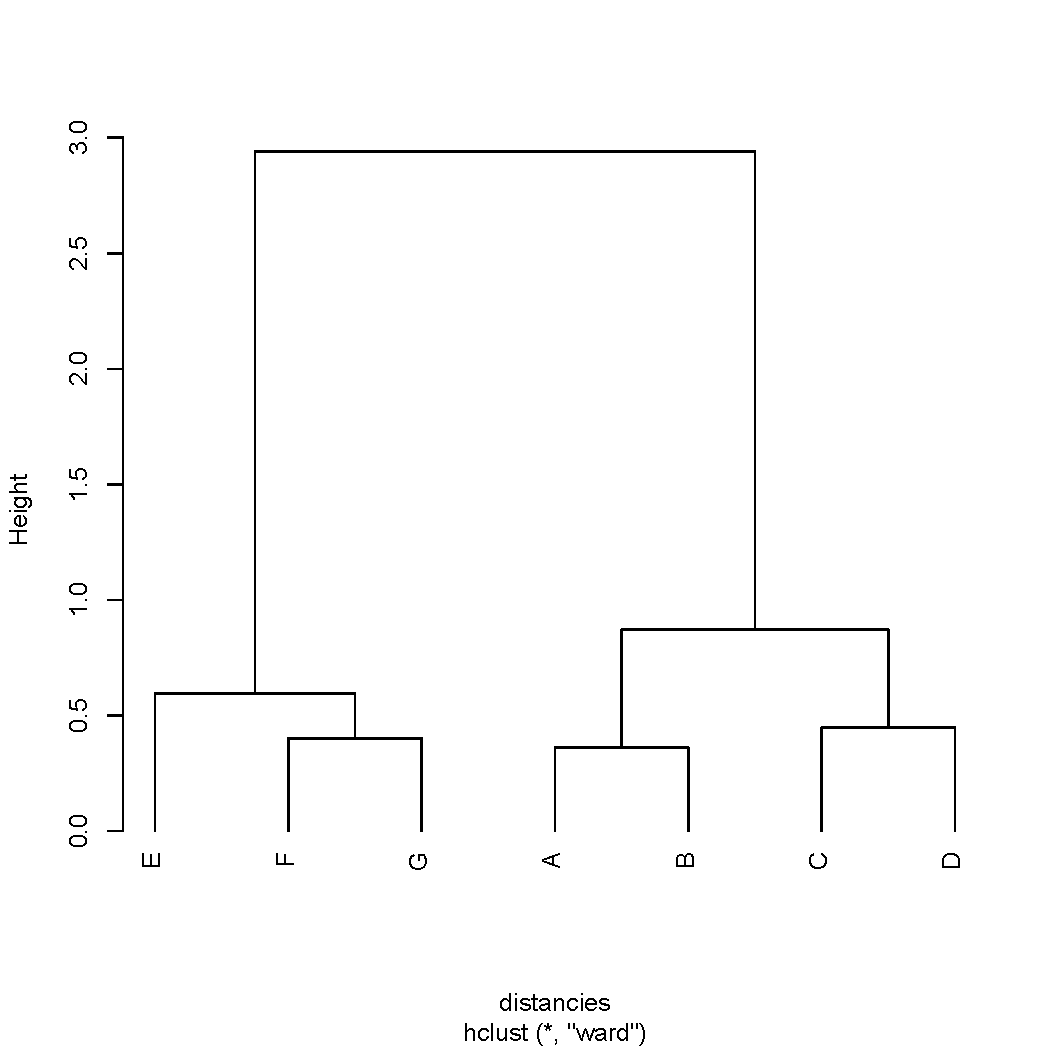
\includegraphics[width=0.7\linewidth]{Rplotw.pdf}
\end{center}
\end{frame}




\begin{frame}
\frametitle{Algunes propietats dels mètodes}
\begin{itemize}
\item El mètode d'enllaç simple, on
$$
d(C,C_1+C_2)=\min \big(d(C,C_1),d(C,C_2)\big),
$$
tendeix a construir clusters grans: clusters que haurien de ser diferents però que tenen dos individus propers s'uneixen en un únic cluster.
\medskip

\item El mètode d'enllaç complet, on
$$
d(C,C_1+C_2)=\max \big(d(C,C_1),d(C,C_2)\big),
$$
se'n va a l'altre extrem, i tendeix a agrupar  clusters només quan tots els punts estan propers.
\end{itemize}
\end{frame}


\begin{frame}
\frametitle{Algunes propietats dels mètodes}
\begin{itemize}
\item El mètode d'enllaç mitjà,
on 
$$
\hspace*{-3ex}d(C,C_1+C_2)=\frac{n_{C_1}}{n_{C_1}+ n_{C_2}} d(C,C_1)+\frac{n_{C_2}}{n_{C_1} + n_{C_2}} d(C,C_2)
$$
és una solució intermèdia.
\medskip

És molt emprat en la reconstrucció d'arbres filogenètics a partir de matrius de distàncies (mètode \emph{UPGMA}, \textsl{Unweighted Pair Group Method Using Arithmetic
averages})

\end{itemize}
\end{frame}

%\begin{frame}
%\frametitle{Algunes propietats dels mètodes}
%
%El mètode de Ward és molt diferent. 
%\medskip
%
%Es defineix l'\emph{heterogeneïtat} d'un cluster $C$ com
%$$
%I_C = \frac{1}{n_C} \sum_{x_i\in C} d^2(x_i,\mathbf{c}_C),
%$$
%on $\mathbf{c}_C$ representa el punt mitjà del cluster $C$ respecte de la distància emprada
%\medskip
%
%Si $d$ és la distància euclidiana, $I_C$ és la variància del cluster $C$
%\end{frame}
%
%\begin{frame}
%\frametitle{Algunes propietats dels mètodes}
%
%Quan dos clusters s'uneixen, 
%$$
%I_{C_1+C_2}=I_{C_1}+I_{C_2}+\frac{n_{C_1}\cdot n_{C_2}}{n_{C_1}+ n_{C_2}} d^2 (C_1,C_2)
%$$
%El mètode de Ward uneix els clusters de manera que l'augment de la suma de les heterogeneïtats sigui mínim.
%\medskip
%
%
%El resultat és que els grups són (globalment) el més homogenis possible.
%\end{frame}
%

\begingroup
\makeatletter
\setlength{\hoffset}{-1\beamer@sidebarwidth}
\makeatother
\begin{frame}[plain]
\begin{center}

\includegraphics[width=1.2\linewidth]{thats-all-folks}
\end{center}
\end{frame}
\endgroup





\end{document}





